\chapter{Quasi-wave/particle Monte Carlo Algorithm, \texorpdfstring{$\varphi MC$}{phiMC}}\label{sec:phase}

\section{Introduction}\label{sec:besintro}

Complex shaped light beams have been used in a wide variety of applications in biophotonics and medicine.
From using Airy beams to move particles and cells~\cite{baumgartl2008optically}, Bessel beam ``tractor beams''~\cite{ruffner2012optical}, Airy and Bessel beams for better field of view in light-sheet microscopy~\cite{vettenburg2014light}, and utilising Laguerre-Gaussian beams to optical trap optically reflective particles~\cite{simpson1996optical}.


However, simulation techniques for modelling complex shaped beams in biological tissue is lacking.
Currently there are several techniques that can model these beams in biological tissue, however they all have downsides.
These methods include diffusion approximation to the~\gls*{rte}, \gls*{fdtd}, \gls*{pstd}, \gls*{bpms}, and \gls*{mcrt}.

As discussed in~\nameref{sec:diffusionapprox} section, the diffusion approximation has many issues when it comes to modelling light propagation in biological tissue.
\gls*{fdtd} involves using a finite difference method to solve Maxwell's equations.
This is computationally intensive and requires a grid resolution of $\sim \lambda/20$ and thus most models are restricted to 2D~\cite{glaser2016fractal,elmaklizi2015penetration}. 
\gls*{pstd} like the \gls*{fdtd} is also computationally intensive, though to a lesser extent~\cite{glaser2016fractal}.
\Gls*{bpm} is a fairly computational efficient method of propagating light beams, compared to~\gls*{fdtd} or~\gls*{pstd}.
However, the~\gls*{bpm} uses the slowly varying envelope approximation, which limits some of the problems it can be applied.
\Gls*{bpm} is also generally a unidirectional propagation method, though it can be adapted to model bidirectional propagation, this can lead to issues in the model's accuracy~\cite{van1981beam,glaser2016fractal}.

\medskip

The final method,~\gls*{mcrt}, in general, cannot model complex beams where the wave-like behaviour of photons is required to form, or propagate the beam.
For example, traditional \gls*{mcrt} methods cannot model Gaussian beams, as Gaussian beams have a finite beam waist at their focus (see~\cref{fig:gbeamills}).
\Gls*{mcrt} (along with geometric optics) predicts that Gaussian beams have an infinitely small waist.

Various authors have tried to model complex beams that require wavelike behaviours using~\gls*{mcrt}.
Some of the techniques used by these authors include: artificial beam steering~\cite{hokr2015modeling}, generating skew rays~\cite{arnaud1985representation}, complex ray tracing~\cite{harvey2015modeling}, decomposition~\cite{worku2018decomposition}, electric field Monte Carlo~\cite{cai2014electric}, and wavefront tracing~\cite{volpe2017huygens}.
However, all these techniques either inaccurately model Gaussian beams, can model Gaussian beams but are complex to implement or computational intensive (more so than \gls*{mcrt} usually is).
There have been some attempts at using the techniques presented in this chapter, to modify MCRT algorithms into algorithms that can model diffraction and interference~\cite{mignon2016fractional,peter2014combining,mahan2018monte,mout2016simulating,fischer2008monte}.
These authors have good results, but either do not detail their methods, do not attempt to treat scattering or are in the x-ray regime.


This chapter modifies the MCRT method, from a ``ballistic'' photon method into a quasi-ballistic/wave photon method so that the wave behaviour of photons can be modelled.
This algorithm, $\varphi MC$, allows the modelling of complex shaped beams such as Bessel beams and Gaussian beams, without much modification of the underlying \gls*{mcrt} code.

We present a thorough investigation of the method used to turn a ballistic regime~\gls*{mcrt} method in to a quasi-wave/ballistic method.
The method is validated against theoretical and experimental data for various different beam types including: Bessel (including higher orders), and Gaussian beams.
Treatment of the propagation through scattering media is also discussed.
The code used in this chapter can be found at: \url{https://github.com/lewisfish/pMC}.


\section{Theory}\label{sec:bestheory}

To convert a MCRT simulation to be able to model wave-like behaviour of photons, we introduce two concepts: tracking the complex phase of packets and the Huygens-Fresnel principle.
This section presents a description of the modifications to the traditional MCRT algorithm, alongside the theoretical background to both the concepts.

\subsection{Complex Phase Tracking}

The first concept we add to the MCRT method is assigning a complex phase to each packet.
The phase is given to a packet at the beginning of the simulation depending on the input field.
The packet is also given an initial electric field of the form:

\begin{equation}
E_0 = \frac{1}{N}\sqrt{\frac{P}{A}}
\label{eqn:initefield}
\end{equation}

Where $N$ is the number of packets run in a simulation, $P$ is the power of the incident beam, and $A$ is the area of the beam.
This initial electric field is needed to compare different beams as in~\cref{sec:compBeams}, and to normalise for number of packets run.

The phase is then tracked as the packet moves through the medium, over a distance $l$.
~\Cref{eqn:phase} shows how the phase is calculated.

\begin{equation}
    \varphi = cos\left(\frac{2 \pi l}{\lambda}\right) + i\ sin\left(\frac{2 \pi l}{\lambda}\right)
    \label{eqn:phase}
\end{equation}

Where $\varphi$ is the complex phase of a photon packet, $l\ [m]$ is the distance the packet has travelled, $\lambda~[m]$ is the wavelength of the packet.
Now we can calculate the complex phase of a packet at a position $P_o$, if we know the distance it has travelled, and its original phase, see~\cref{fig:phase-diag}.

\begin{figure}[!htbp]
    \centering
    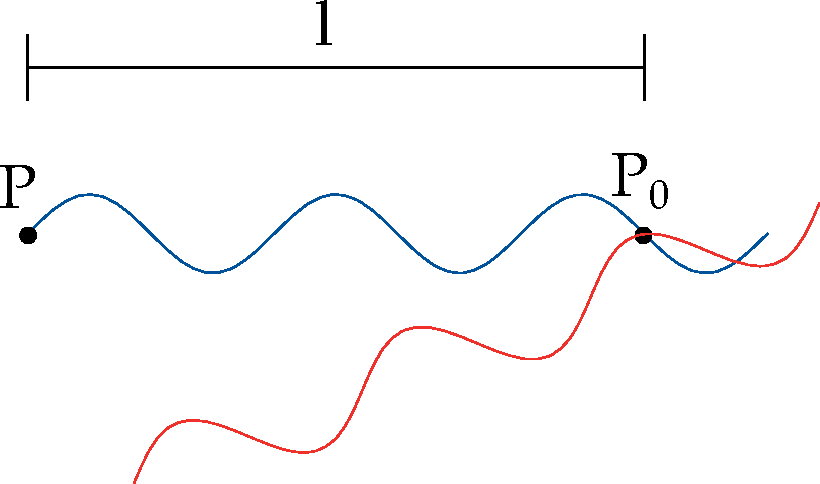
\includegraphics[width=0.5\textwidth]{phase-diag.pdf}
    \caption{Example of phase calculation when a photon has travelled a distance l. The figure also shows an example of interference between two photons via addition of the complex amplitudes at the point $P_0$.}
    \label{fig:phase-diag}
\end{figure}

To model interference, we let the photon packets interfere with one another in a volume or area element. 
We do not model the interference at a point in space where photon packets cross, due to the ballistic nature of the \gls*{mcrt} simulation this does not occur with enough frequency to give a good signal to noise ratio. 
Therefore, interference takes place in a volume, $dV$, or area element, $dA$, instead.
To calculate the intensity from the complex phase, the absolute value of the phase is squared.
Therefore, to calculate the intensity for a given voxel or area, the phase is first summed in each voxel or area before the absolute value is squared.~\Cref{eqn:intense} shows the equation for intensity for a volume element $dV$. A similar relation for calculating the interference on an area element $dA$ also exists.

\begin{equation}
I(\zeta)= \left| \sum\limits_{\zeta}E_0\ cos\left(\frac{2\pi l}{\lambda}\right) + i \sum\limits_{\zeta}E_0\ sin\left(\frac{2\pi l}{\lambda}\right)\right|^2,\ \ \ \zeta=(x,y,z)
\label{eqn:intense}
\end{equation}

\noindent Where:

\indent $l$ is the total distance travelled by a photon [$m$];

\indent $\lambda$ is the wavelength of the photon [$m$];

\indent $I$ is the intensity at the $\zeta^{th}$ cell [$W m^{-2}$];

\indent $E_0$ is the initial electric field of the packets as in~\cref{eqn:initefield} [$Vm^{-1}$]

\indent and $\zeta$ is $x^{th}$, $y^{th}$, $z^{th}$ cell, volume $dV$.

\medskip

In addition to tracking the phase, the next principle needed to simulate the wave behaviour of light in MCRT is the Huygens-Fresnel principle.

\subsection{Huygens-Fresnel Principle}

The Huygens-Fresnel principle is a method that is used to help model the propagation of waves in the far field limit and the near field limit. 
The Huygens principle was first postulated in 1678 and states~\cite{huygens2012treatise,hecht2017optics,huygens1900wave}: 

\medskip

``\textit{Every point on a propagating wavefront serves as the source of spherical secondary wavelets, such as the source at some time later is the envelope of these wavelets.}''

\medskip

The principle is illustrated in~\cref{fig:huygensillis}.
The principle allowed Huygens to derive laws of refraction and reflection, but it failed to describe diffraction effects.
This led to Augustin-Jean Fresnel in 1818, combining the Huygens principle with his own theory of interference~\cite{fresnel1819memoire,huygens1900wave}.
This Huygens-Fresnel principle gave an accurate description of the propagation of light and diffraction effects.
This was achieved by allowing the secondary wavelets to self interfere, giving rise to an accurate description of the physical phenomena.
Later, Gustav Kirchhoff gave a rigours mathematical description of the Huygens-Fresnel principle, which is the basis of diffraction theory~\cite{kirchhoff1883ann,born2000principles}. 

\begin{figure}[!htbp]
    \centering
    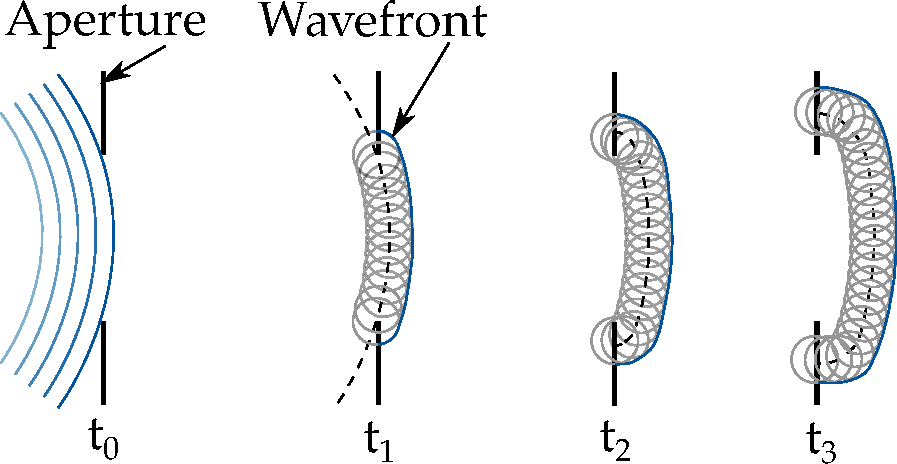
\includegraphics[width=0.6\textwidth]{huygens.pdf}
    \caption{Illustration of the Huygens-Fresnel principle. At $t_0$ a wave is incident on an aperture. Times $t_1,\ t_2,\ \text{and}\ t_3$ show the evolution of the wavefront using the Huygens-Fresnel principle. Dashed lines illustrate the wavefront position at the previous time step and is the source of the Huygens-Fresnel wavelets.}
    \label{fig:huygensillis}
\end{figure}

The Huygens-Fresnel principle allows the modelling of diffraction in both the near and far field.
As the principle states that every point on the wavefront is a source of secondary spherical waves, this implies that there are ``backward'' waves.
These ``backward'' waves are un-physical, and there is no experimental evidence of their existence.
Thus, Fresnel introduced an inclination factor to eliminate these ``backward'' waves.
This inclination factor was later put on a rigorous mathematical standing by Kirchoff, as it naturally fell out of his theory~\cite{kirchhoff1883ann,born2000principles}.
\Cref{eqn:kirchhoffeqn}, the Rayleigh-Sommerfeld diffraction integral of the first kind\footnote{If diffraction occurs in a plane, the Kirchoff diffraction integral can be modified to this}, shows the equation for the complex field at a point on a plane.

\begin{equation}
u(\mathbf{r_1})=\frac{1}{i\lambda}\int\int u(\mathbf{r_0})\frac{\mathbf{\hat{s_0}} \cdot (\mathbf{r_1} - \mathbf{r_0})}{\left|\mathbf{r_1} - \mathbf{r_0}\right|^2}e^{ik\left|\mathbf{r_1} - \mathbf{r_0}\right|}dS_0
\label{eqn:kirchhoffeqn}
\end{equation}

\noindent Where:

    \indent $u$ is the complex electric field [$Vm^{-1}$];

    \indent $\lambda$ is the wavelength [$m$];

    \indent $S_0$ is a plane with surface normal $\mathbf{\hat{s_0}}$ [-];

    \indent $k$ is the wavenumber [$m^{-1}$];

    \indent and $\mathbf{r_n}$ are spatial coordinates [-]. 

\medskip

The Huygens-Fresnel principle is implemented by sampling the light source on the surface of any lens or in a slit.
In practice this means when for example, a plane wave is incident on a slit width \textit{a}, and length \textit{b}, the slit area is uniformly sampled for the initial position of the photon packets.
The packets are then given a random direction, sampled toward the detector thus avoiding the non-existent ``backward'' waves.
For the case of modelling propagation through a lens, the usual geometric optics approach is taken to propagate the packets through the lens.
When the packet lies on the surface of the lens, the Huygens-Fresnel principle is invoked, and the packet is given a random direction (in the direction of the medium) and propagated as usual.

\medskip

Our algorithm uses the Huygens-Fresnel principle and the tracking of complex phase to simulate diffraction effects, that would otherwise be absent from the simulation.
The principle allows the algorithm to calculate the complex amplitude at a point, and thus the intensity at that point, essentially numerically simulating~\cref{eqn:kirchhoffeqn}.
These two concepts underpin the algorithm that allows various complex beams, and wave phenomena to be simulated within a ballistic method. The following sections validate the method against the theory and experimental data for propagation of various complex beams.


\subsection{Validation of Phase Tracking Algorithm}

\subsubsection*{Double Slit Experiment}

The first test of our quasi-wave/particle MCRT algorithm\footnote{Though this example is not strictly MCRT, but rather ray tracing, as it involves no scattering. The full MCRT method will be used in later sections.}, $\varphi MC$, is to compare our simulation to a double slit experiment.
The double slit experiment is a simple experiment where a monochromatic plane wave of light is incident on two slits distance apart $d$, and width $b$, and an interference pattern is observed on a screen a distance $L$ away from the slits. The experiment is usually carried out with the detector screen in the far field (the so called Fraunhofer regime).
The intensity pattern on the detector screen is as in~\cref{eqn:doubleslit}:

\begin{equation}
    I(x) \propto cos^2\left(\frac{kdx}{2\sqrt{L^2+x^2}}\right)sinc^2\left(\frac{kax}{\sqrt{L^2+x^2}}\right)
    \label{eqn:doubleslit}
\end{equation}

Where the $sinc$ function is defined as $\tfrac{sin(x)}{x}$, for $x\ \neq 0$, $k$ is the wavevector, $k=\tfrac{2\pi}{\lambda}$, and $x$ is the horizontal position on the detector screen.

The simulation was carried out for a wavelength, $\lambda$,  of $488~nm$, a slit width of $10\lambda$, slit separation of $80\lambda$, and the detector screen positioned $10000\lambda$ away from the slits.
Using the Huygens-Fresnel principle, each slit is a source of Huygens wavelets.
The detector screen has dimensions, $1~mm^2$ and there are $2051^2$ bins, giving a bin an effective size: $\sim 488~nm$ or $\sim \lambda$.
The initial position of the photon packets is sampled uniformly from the slit area, after randomly choosing one of the slits to emit from.
A random direction is then chosen to ensure that the packets will hit the detector screen.
The simulation was run with $10^9$ packets, which took $\approx10~mins$ to run on an 8 core Intel Xeon machine.
This gave an accurate match to the theoretical expression, as seen in~\cref{fig:doubleslitcomp}.

\begin{figure}[!htbp]
    \centering
    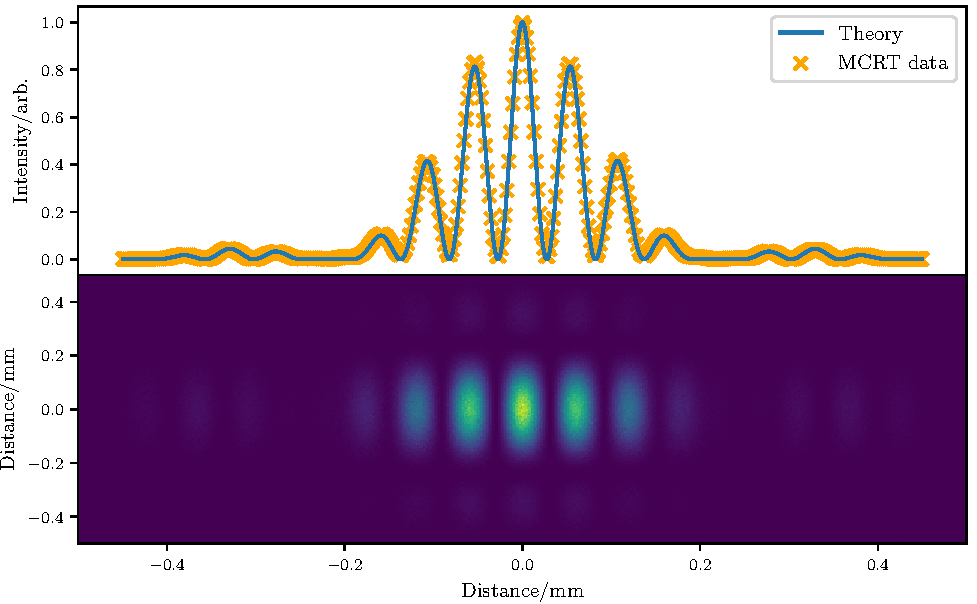
\includegraphics[width=0.75\textwidth]{doubleslit.pdf}
    \caption{Comparison of theory and simulation for the double slit experiment. Top image shows a slice through the computed image and the expected profile from theory. For clarity only every $5^{th}$ MCRT data point is plotted. Bottom image shows the computed image.}
    \label{fig:doubleslitcomp}
\end{figure}

\subsubsection*{Diffraction by a Square Slit}
$\varphi MC$ is also validated by simulating diffraction from a square aperture in the far and near field. 
Fresnel diffraction occurs in the near field when the \textit{Fresnel number},~\cref{eqn:fnumber}, is greater than 1.0.
Fraunhofer diffraction occurs when the \textit{Fresnel number} is less than 1.0.

\begin{equation}
F = l\sqrt{\frac{2}{\lambda r_0}}
\label{eqn:fnumber}
\end{equation}

\Cref{eqn:fnumber} is the Fresnel number, where \textit{l} is the slit width, $\lambda$ is the wavelength of the incident radiation, and $r_0$ is the distance from the aperture to the detector screen, as shown in~\cref{fig:aperture}. 

\medskip
\begin{figure}[!htbp]
    \centering
    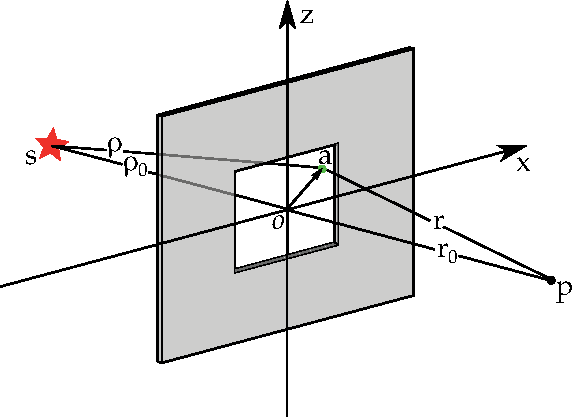
\includegraphics[width=0.75\textwidth]{aperture.pdf}
    \caption{Geometry of the square aperture used in the validation.}
    \label{fig:aperture}
\end{figure}

To compare $\varphi MC$ to the theory, the theory must first be discussed.
Consider the setup as shown in~\cref{fig:aperture}, to calculate the intensity at a point $P$ the contribution by an area element $dS$ at the point $a$, to the optical disturbance at a point \textit{P} is considered.
Accounting for the unobstructed optical disturbance from $S$ as well and using~\cref{eqn:kirchhoffeqn}, yields: 


\begin{equation}
U(P)=\frac{1}{i\lambda}\iint\limits_{\Sigma} \frac{Ae^{i(k\rho-\omega t)}}{\rho} \frac{e^{ikr}}{r}cos(\theta)\ dS
\label{eqn:disturb}
\end{equation}


In the case where $\rho_0$ and $r_0$ are large compared to the size of the aperture, then $\cos\left(\theta\right) = 1$ and $\tfrac{1}{\rho r}=\tfrac{1}{\rho_0 r_0}$.
The lengths of $r_0$ and $\rho_0$ are:

\begin{align}
r=&\sqrt{r_0^2+y^2+z^2}\label{eqn:r} \\
\rho=&\sqrt{\rho_0^2+y^2+z^2}\label{eqn:rho}
\end{align}

Using the binomial theorem to expand~\cref{eqn:r,eqn:rho} yields:

\begin{equation}
\rho + r \approx \rho_0 + r_0 + (y^2+z^2)\frac{\rho_0r_0}{2\rho_0r_0}
\label{eqn:binomial}
\end{equation}

Substituting~\cref{eqn:binomial} into~\cref{eqn:disturb} with $k=2\pi/\lambda$

\begin{equation}
U(P)=\frac{Ae^{-i[k(\rho_0+r_0)\omega t]}}{i\lambda\rho_0r_0}\iint\limits_{\Sigma} e^{i2\pi y^2\tfrac{(\rho_0+r_0)}{2\lambda\rho_0r_0}+i2\pi z^2e^{\frac{i\pi u^2}{2}}\tfrac{(\rho_0+r_0)}{2\lambda\rho_0r_0}} \ dS
\label{eqn:midway}
\end{equation}


Introducing the dimensionless variables \textit{u} and \textit{v}

\begin{align}
u&=y\sqrt{\frac{2(\rho_0+r_0)}{\lambda\rho_0r_0}}\\
v&=z\sqrt{\frac{2(\rho_0+r_0)}{\lambda\rho_0r_0}}
\end{align}

and substituting them into~\cref{eqn:midway}.

\begin{equation}
U(P)=\frac{\tilde{E}_u}{2}\int_{u_1}^{u_2} e^{\tfrac{i\pi u^2}{2}}\ du\int_{v_1}^{v_2} e^{\tfrac{i\pi v^2}{2}} \ dv
\label{eqn:pentdisturb}
\end{equation}
\Cref{eqn:pentdisturb} describes the optical disturbance at the point $P$, with $\tilde{E}_u$ the unobstructed disturbance at $P$.
\Cref{eqn:pentdisturb} can be evaluated using the Fresnel integrals, $C(w)$ and $S(w)$:


\begin{equation}
\int_{0}^{w}e^{i\pi w'^2/2}dw'=C(w)+iS(w)
\label{eqn:fresneleqn}
\end{equation}


\begin{align}
S(w)&=\int^w_0 sin\left(\frac{\pi w'^2}{2}\right)dw'\label{eqn:fresint1}\\
C(w)&=\int^w_0 cos\left(\frac{\pi w'^2}{2}\right)dw'\label{eqn:fresint2}
\end{align}


Using~\cref{eqn:fresneleqn}, where $C(w)$ and $S(w)$ are the Fresnel integrals as in~\cref{eqn:fresint1,eqn:fresint2}.
\Cref{eqn:pentdisturb} can then be transformed into an intensity, by taking the absolute value and squaring, yielding~\cref{eqn:fresIntensityp}:


\begin{equation}
I_p = \frac{I_u}{4} \{[C(u_2) - C(u1)]^2 + [S(u_2) - S(u_1)]^2\} \times \{[C(v_2) - C(v_1)]^2 + [S(v_2) - S(v_1)]^2\}
\label{eqn:fresIntensityp}
\end{equation}

\Cref{eqn:fresIntensityp} gives the intensity of the field at the point $P$ on axis for a square aperture where $I_u$ is the unobstructed intensity at the point $P$. 

\medskip

As the mathematics of calculating the optical disturbances at all points on a plane at point $P$ is difficult, instead the aperture is moved by small displacements, with $\overrightarrow{SOP}$ fixed.
This effectively achieves the translation of the origin, $O$, with respect to the fixed aperture. 
Thus, for each displacement new aperture coordinates $y_1$, $y_2$, $z_1$, and $z_2$ are generated and therefore new $u_1$, $u_2$, $v_1$, and $v_2$.
Therefore, the intensity at a point $P +\delta d$, where $\delta d$ is the displacement, can be calculated.
This approximation holds for displacements that are small compared to the $\rho_0$~\cite{born2000principles,hecht2017optics,goodman2017introduction}.
Using this method and~\cref{eqn:fresIntensityp} gives the theoretical curves in~\cref{fig:frescompare}.

\medskip

In $\varphi MC$, the above experiment is simulated. 
A square slit is uniformly sampled in the $x$, and $z$ direction to get the packets initial position. 
A random direction is then sampled, by uniformly picking a point on the detector screen.
This ensures the algorithm does not waste time by calculating packets trajectories that are not registered by the detector.
We assume a plane wave is incident on the aperture and each photon is given the same initial complex electric field.

The distance between the detector screen and the aperture is varied and the intensity on the screen is measured for $\sim 10^{10}$ photons released from the aperture as Huygens wavelets.
For \textit{Fresnel numbers} greater than 1.0, the number of bins is 300, covering a distance of 600~$\mu m$. 
For the case of Fraunhofer diffraction, the number of bins is 100 covering a distance of 6000~$\mu m$.
The simulations take $\sim$ 3 minutes for $10^{10}$ packets to be run on an Intel Xeon E3--1245 v5, 8 cores @ 3.5GHz machine.
The number of bins and photons packets simulated had to be increased for the cases where the Fresnel number was large (i.e the detector screen was near the aperture).
This is due to the diffraction pattern becoming ``noisy'' and thus needs a higher resolution to accurately simulate.
\cref{fig:frescompare} shows the comparison between the theory and the $\varphi MC$ simulations.

\begin{figure}[!htbp]
    \centering
    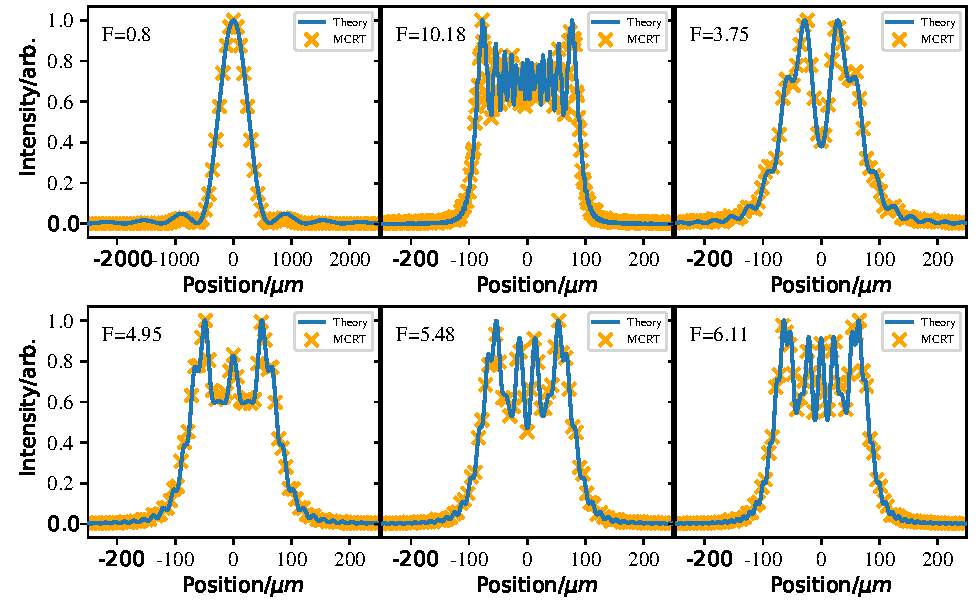
\includegraphics[width=0.95\textwidth]{Fresnel-compare.pdf}
    \caption{Comparison of theory and simulation for diffraction through a square aperture in the Fresnel and Fraunhofer regimes.}
    \label{fig:frescompare}
\end{figure}

\FloatBarrier
\newpage
\section{Gaussian Beams}

Now that the method of tracking the complex phase of packets and using the Huygens-Fresnel principle has been verified against theoretical results, we can now turn our attention to modelling the propagation of beams that require the wave behaviour of light to either form or propagate.
The first beam type we will examine is the Gaussian beam.
Gaussian beams are important as most laser beams have the profile of the fundamental (TEM$_{00}$) Gaussian mode.
This section will show that $\varphi MC$ can accurately model all the physical phenomena of Gaussian beams, within the \gls*{mcrt} regime.

Before discussing how $\varphi MC$ can model a Gaussian beam, the theory and various physical parameters of the beam must be described. 
The electric field of a Gaussian beam can be defined as in~\cref{eqn:gaussefield}~\cite{milonni2010laser}:

\begin{equation}
E(r,z)=E_0\frac{w_0}{w(z)}e^{\frac{-r^2}{w(z)^2}}e^{-i(kz+k\frac{r^2}{2R(z)}-\varphi(z))}
\label{eqn:gaussefield}
\end{equation}

\noindent Where:

    \indent $r$ is the radial distance from the optical axis [$m$];

    \indent $z$ is the axial distance from  the beam waist [$m$];

    \indent $k$ is the wavenumber $k=\frac{2\pi}{\lambda}$ [$m^{-1}$];

    \indent $E_0$ is the electric field amplitude at the origin [$Vm^{-1}$];

    \indent $w(z)$ is the radius of the beam at which the amplitude has fallen to $\frac{1}{e}$, at the distance $z$ along 

    \indent the beam,~\cref{eqn:gwaist} [$m$];

    \indent $w_0$ is the waist radius [$m$];

    \indent $R(z)$ is the radius of curvature of the beam's wavefronts at $z$,~\cref{eqn:radiuscurve} [$m$];

    \indent and finally, $\varphi(z)$ is the Gouy phase at $z$,~\cref{eqn:gouyphase} [-].

\medskip

~\Cref{eqn:gwaist,eqn:gouyphase,eqn:rayleighrange,eqn:beamwaist,eqn:radiuscurve} give the definitions of key physical properties as outlined above or as shown in~\cref{fig:gbeamills}. 
$z_r$ is the Rayleigh range,~\cref{eqn:rayleighrange}, and defines the point at which the beam's waist grows to $\sqrt{2}$ times the size of the beam at its waist.
The waist of the beam at the focal point is defined as~\cref{eqn:beamwaist}, where $f$ is the focal length and $D$ is the $\tfrac{1}{e^2}$ diameter of the beam at the lens.

\begin{align}
    w(z) &= w_0\sqrt{1+\left(\frac{z}{z_r}\right)^2} \label{eqn:gwaist} \\
    R(z) &= z\left[1+\left(\frac{z_r}{z}\right)^2\right]\label{eqn:radiuscurve}\\
    \varphi(z) &= arctan\left(\frac{z}{z_r}\right)\label{eqn:gouyphase}\\
    z_r &= \frac{\pi w_0^2}{\lambda}\label{eqn:rayleighrange}\\
    w_0 &= \frac{2\lambda f}{\pi D}\label{eqn:beamwaist}\\
\end{align}

\begin{figure}[!htbp]
    \centering
    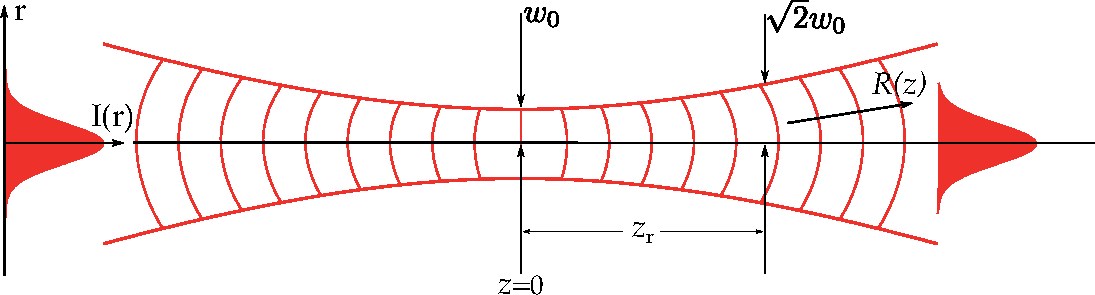
\includegraphics[width=0.95\textwidth]{gaussian-radius-curve.pdf}
    \caption{Illustration of a Gaussian beam focusing to its waist then diverging away. Image shows the various defined properties of a Gaussian beam along side the radius of curvature changing direction at the waist.}
    \label{fig:gbeamills}
\end{figure}

With the physical properties of the Gaussian beam outlined, a Gaussian beam can now be modelled using our algorithm.
To simulate a Gaussian beam, we set up the simulation as shown in~\cref{fig:gausssetup}.
The simulated lens used is a convex-plano lens, with a radius of curvature, $4.6~mm$, thickness, $L_t$, of $2.2~mm$, and working distance, $W_d$, 8.5~$mm$.
A Gaussian beam wavelength $488~nm$ and $\tfrac{1}{e^2}$ waist diameter $0.5~mm$, is incident on the lens.
Using~\cref{eqn:beamwaist} yields the size of the focal spot as $3.1~\mu m$.

\begin{figure}[!htbp]
    \centering
    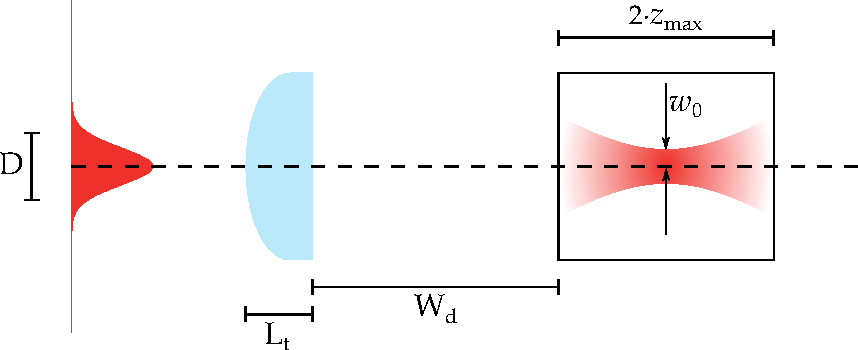
\includegraphics[width=0.75\textwidth]{gaussiansetup.pdf}
    \caption{Simulation setup of focusing a Gaussian beam through a lens. Lens is convex-plano and is modelled on ThorLabs LA4249 UV fused silica lens~\cite{thorlens}.  $L_t$ is the lens thickness, D is the $\tfrac{1}{e^2}$ input beam diameter, $W_d$ is the working distance or back focal length, $2 \cdot z_{max}$ is the depth of the medium, and $w_0$ is the beam waist.}
    \label{fig:gausssetup}
\end{figure}

To model the lens in $\varphi MC$ the photons initial $z$ position is set just in front of the lens.
The $x$ and $y$ are randomly sampled from a Gaussian distribution with a waist of $\sqrt{2}w_0$.
The factor of $\sqrt{2}$ accounts for the conversion from intensity to electric field beam waist.
This is because the electric field is $\propto \exp{\left(\tfrac{-r^2}{4\sigma'^2}\right)}$, and the intensity is $\propto \exp{\left(\tfrac{-r^2}{2\sigma^2}\right)}$.
Thus, for the input electric field waist to be equal to the intensity,  $\sigma'=\sqrt{2}\sigma$.
The packet is given an electric field of the form~\cref{eqn:initefield}, with $P=1~mW$, and $A=\tfrac{1}{2}\pi w_0^2$.

The packet is then propagated to the surface of the convex side of the lens.
This is achieved by finding the intersection of a sphere, which represents the convex side of the lens, and the packets path.
With the packet on the surface of the lens, Fresnel coefficients are calculated to determine if the packet is reflected or refracted.
If the packet is reflected, the packet is killed and the process starts again.
If the packet is refracted, the packet is moved into a new direction on the planar surface of the lens.
The new direction vector is calculated using a vector version of Snell's law (see~\cref{app:fresnelappend} for a discussion of this).
The packets are then uniformly sampled onto the surface of the voxel medium and the usual~\gls*{mcrt} method is used to propagate the packet whilst tracking the phase.

\begin{figure}[!htpb]
    \centering
    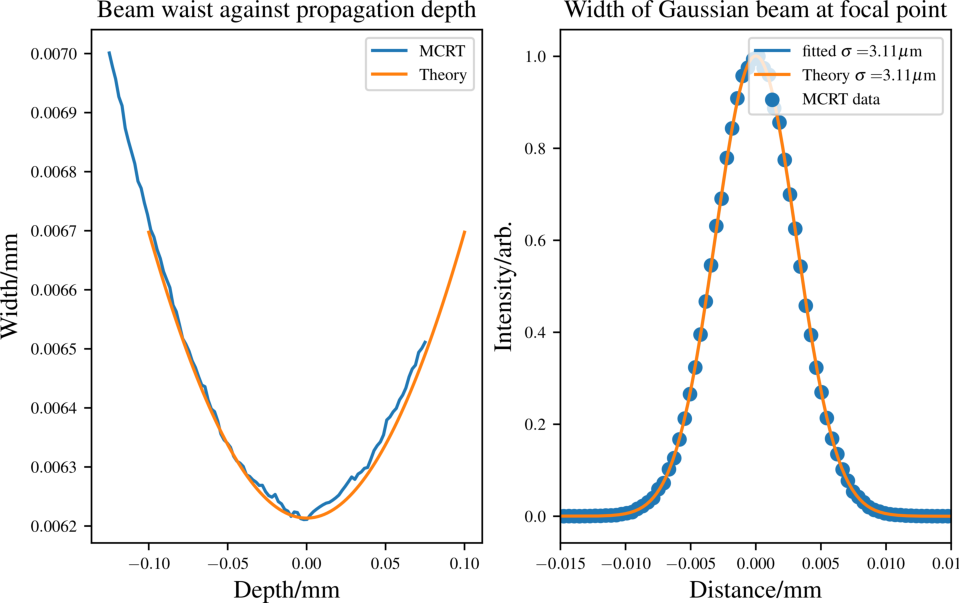
\includegraphics[width=0.75\textwidth]{gaussian.pdf}
    \caption{Results of \textit{in-silico} experiment of focusing a Gaussian beam through a convex-plano lens.}
    \label{fig:simgaussexp}
\end{figure}


\Cref{fig:simgaussexp} shows the comparison of theory and \textit{in-silico} experiment, with excellent agreement between the two.

$\varphi MC$ also correctly models the change of direction of the radius of curvature, $R(z)$, as is predicted by theory.
This process is described by~\cref{eqn:radiuscurve}, before the waist the curvature is negative, at the waist it is infinite, and past the waist its is positive.
This can be seen in~\cref{fig:proofchgrz}, where the beam (direction of propagation right to left) undergoes this:

\begin{figure}[!htpb]
    \centering
    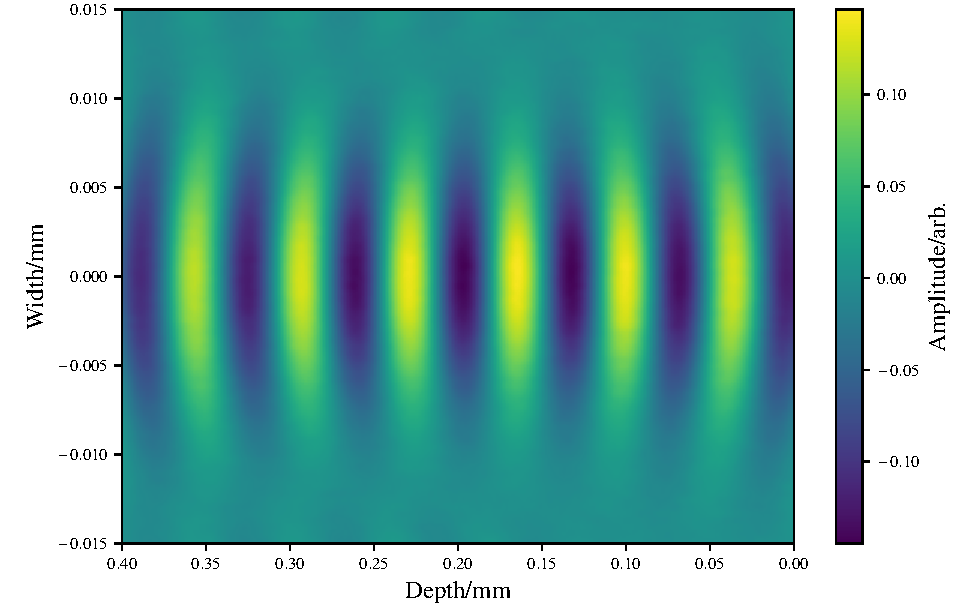
\includegraphics[width=0.75\textwidth]{radcurvechange.pdf}
    \caption{Slice through the real part of the complex electric field of the \textit{in-silico} experiment as in~\cref{fig:gausssetup}. Figure shows the radius of curvature changing direction at the waist as predicted by theory.}
    \label{fig:proofchgrz}
\end{figure}

$\varphi MC$ can also model spherical aberrations caused by lenses.
\Cref{fig:spheraberr} shows aberrations caused by a plano-convex lens alongside an illustration of the paths that light take through the imperfect lens, causing spherical aberrations.

\begin{figure}[!hbtp]
    \centering
    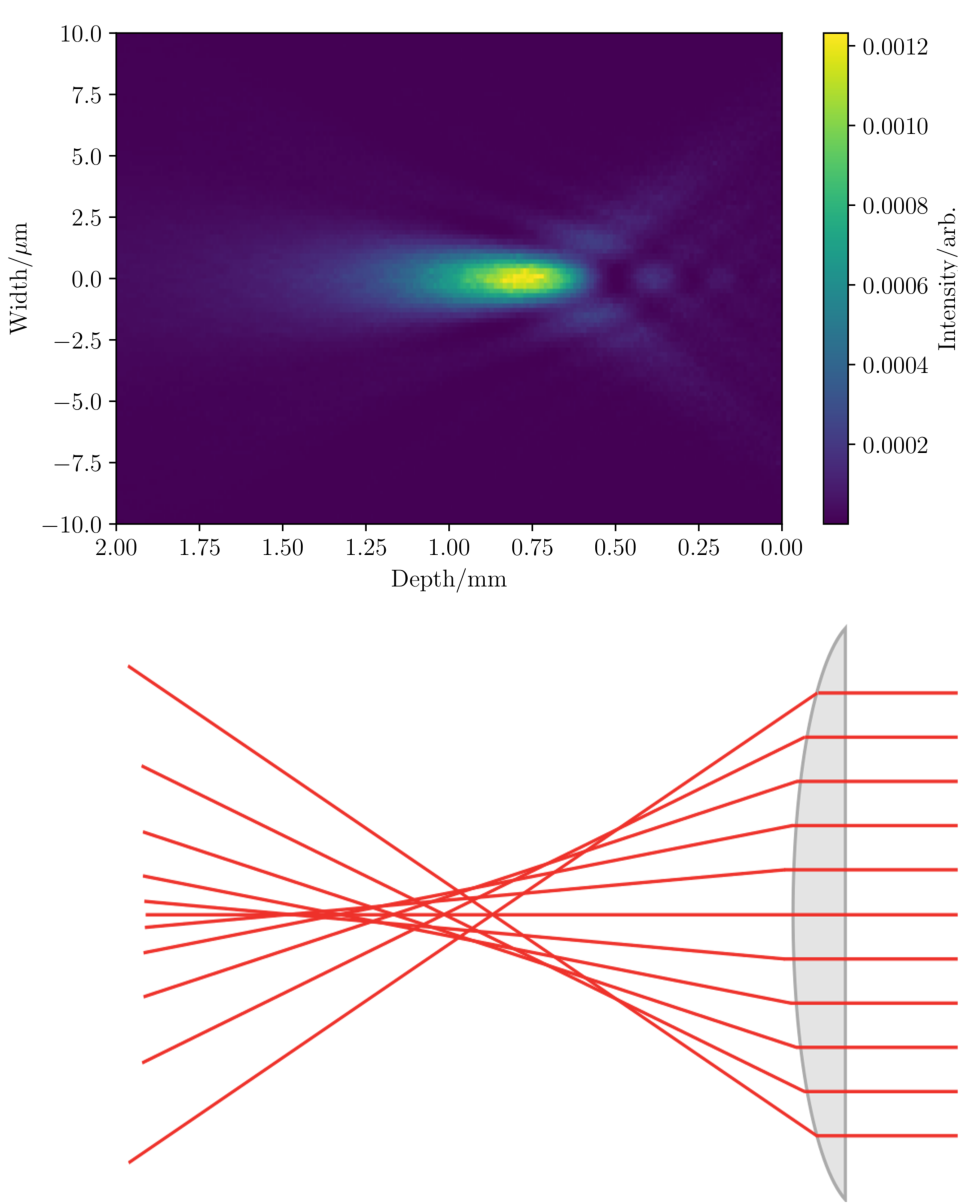
\includegraphics[width=0.65\textwidth]{spher-aber.pdf}
    \caption{Illustration of $\varphi MC$'s ability to model spherical aberrations. Top image generated using the same setup as in~\cref{fig:gausssetup}, but with $D=1.5~mm$ within $\varphi$MC. Image shows the elongated focus and characteristic interference pattern behind the focus. Bottom image shows an illustration of rays traced through a lens which suffers from spherical aberration.}
    \label{fig:spheraberr}
\end{figure}


This section has shown that Gaussian beams, and their physical phenomena can be accurately modelled using $\varphi MC$.
A convex-plano lens was used to focus a Gaussian beam, but it is simple to implement other lenses given a triangulated mesh of the lens or an equation that describes the shape of the lens, e.g an aspheric lens.
\FloatBarrier

\section{Bessel Beams}

Bessel beams have been the subject of intense research since their discovery in 1987~\cite{durnin1987diffraction,durnin1987exact}. 
Durnin noticed that the solution to the Helmholtz equation of the Bessel type were independent of the direction of propagation.
This means that the central core of the beam is generally more diffraction resistant when compared to a Gaussian beam with a similar spot size.
Bessel beams also have a property of ``self-healing'', this means if an obstruction is placed in the path of the central lobe of the Bessel beam, the Bessel beam can then ``heal'' and reform past the obstruction~\cite{mcgloin2005bessel}.
However, it is physically impossible to create a ``real'' Bessel beam as the Bessel beam can have infinite rings, which each carry the same amount of power, thus would require an infinite amount of power~\cite{durnin1987diffraction}.
Therefore, all Bessel beams that are created experimentally are quasi-Bessel beams which are similar to their theoretical counterpart over a finite distance~\cite{durnin1987diffraction}.


These two properties make Bessel beams an attractive avenue of research, as novel solutions to imaging problems.
There is also some debate among physicists as to whether these phenomena are justly labelled, or if they glib terms used to make Bessel beams seem better than they are~\cite{debeer1987comment,harvey1984spot,durnin1987reply,sprangle1991comment,durnin1991durnin}.

\subsection{Theory}
As before with the Gaussian beam, the theory behind the Bessel beam must be discussed before we can model the beam in $\varphi MC$.
The electric field can be described using~\cref{eqn:besselEfield}~\cite{vcivzmar2006opticke}:

\begin{equation}
    E(r,z)=E_0\sqrt{\frac{2\pi k z w_0\sin(\beta)}{z_{max}}}\ \text{exp}^{\left(-\frac{z^2}{z_{max}^2}-\frac{i\pi}{4}\right)}\ J_0\left(kr\sin(\beta)\right)\ \text{exp}^{\left(ikz\cos(\beta)\right)}
    \label{eqn:besselEfield}
\end{equation}

\noindent Where:

    \indent $k$ is the wavevector, $k=\tfrac{2\pi}{\lambda}$ [$m$];

    \indent $z$ is the propagated distance [$m$]; 

    \indent $\beta$ is the angle the wavefront propagates at (see~\cref{fig:besselgeo}) [$rad$]; 

    \indent $w_0$ is the $\tfrac{1}{e^2}$ width of the input Gaussian beam [$m$]; 

    \indent $J_0$ is the Bessel function of the first kind, zeroth order; 

    \indent $r$ is radial distance from the optical axis [$m$]. 

\medskip


~\Cref{eqn:besselEfield} gives the electric field for a Bessel beam. The intensity can be calculated using:

\begin{equation}
    I(r,z)=\frac{c\epsilon_0\left|E\right|^2}{2}
    \label{eqn:besselintsub}
\end{equation}

Using the definition total power transmitted by a beam as:

\begin{equation}
    P=\frac{\pi I_0w_0^2}{2}
    \label{eqn:pwrdef}
\end{equation}

Where $I_0$ is defined as on axis intensity of the incident Gaussian beam.

\begin{equation}
    I_0=\frac{c\epsilon_0E_0^2}{2}
    \label{eqn:intdef}
\end{equation}

Substituting~\cref{eqn:besselEfield,eqn:intdef,eqn:pwrdef} into~\cref{eqn:besselintsub} yields:

\begin{equation}
    I(r,z)=\frac{4k_rP}{w_0}\frac{z}{z_{max}}J_0^2\left(k_r\ r\right)\text{exp}^{\left(-\frac{2z^2}{z^2_{max}}\right)}
    \label{eqn:besselInt}
\end{equation}


\noindent Where:

    \indent $k_r$ is the radial wavevector, $k_r=k\ sin(\beta)$;

    \indent $P$ is the power of the incident Gaussian beam.

    \medskip

A Bessel beam can be formed by an axicon lens (see~\cref{fig:besselgeo}) or by diffraction through a ring, or through the use of a spatial light modulator.
All the simulations of Bessel beams in this thesis use the axicon method of generating a Bessel beam, thus only axicons will be discussed.
\Cref{fig:besselgeo} shows the geometry of a Bessel beam formed by an axicon.
Using simple geometry and Snell's law the following equations can be derived to describe various properties of a Bessel beam formed by an axicon~\cite{merola2012characterization}.

The propagation depth of a Bessel beam is defined as the distance from the tip of the axicon to the end of the ``Bessel region''. However, in reality the Bessel beam will continue to propagate slightly passed this depth.
~\Cref{eqn:besselzmax} shows the propagation depth of a Bessel beam where $cot$ is the cotangent function ($cot x = \tfrac{1}{\tan x}$).
\begin{equation}
z_{max}=R\left(cot\left(\beta\right) - tan\left(\alpha\right)\right)
\label{eqn:besselzmax}
\end{equation}

The propagation angle of the conical waves, $\beta$ can be calculated using Snell's law and $\alpha$ the angle of the axicon:

\begin{equation}
\beta = arcsin\left(n\ sin\left(\alpha\right)\right)-\alpha
\label{eqn:betaangle}
\end{equation}

The central core of a Bessel beam is defined as the distance to the first zero of the Bessel beam.
\Cref{eqn:coreradius} shows the radius of the core, where $2.405$ is derived from the position of the first zero of the Bessel function.

\begin{equation}
r_o = \frac{2.405}{k\ sin\left(\beta\right)}
\label{eqn:coreradius}
\end{equation}

Finally, the spacing between Bessel beam rings is:
\begin{equation}
\Delta \rho = \frac{\lambda}{2\ sin\left(\beta\right)}
\end{equation}

\subsection{Validation}

To ensure that the method described in~\cref{sec:bestheory} works as intended for Bessel beams several tests are compared to theoretical expressions and experimental data.
\begin{figure}[!htbp]
    \centering
    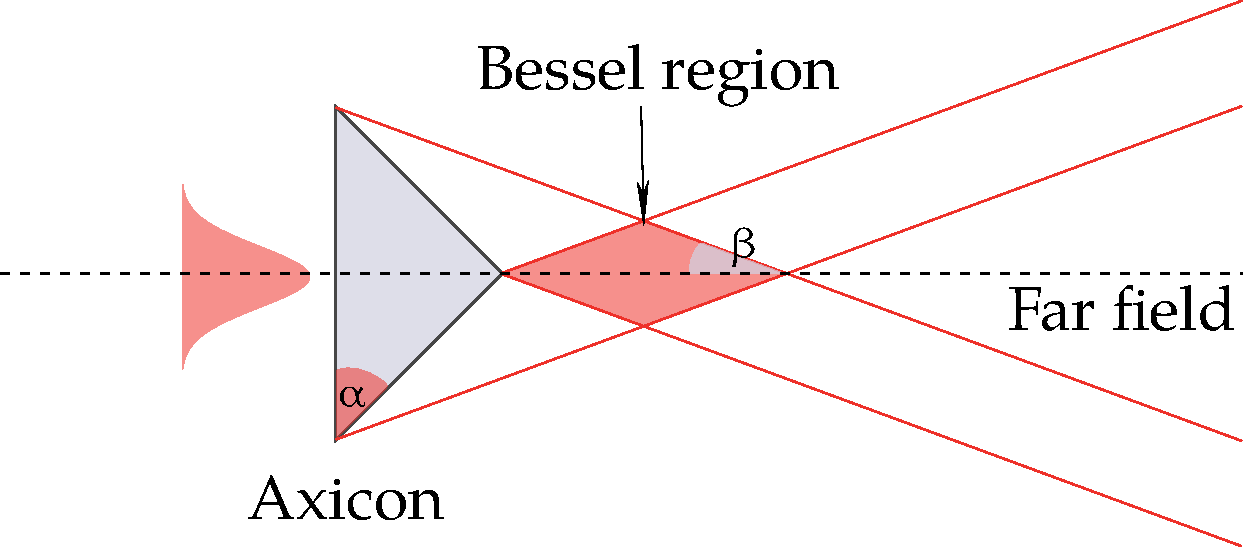
\includegraphics[width=0.5\textwidth]{bessel.pdf}
    \caption{Geometry of a Bessel beam, generated by an axicon lens. $\beta$ is the angle with the optical axis, and the angle of the conical waves. $\alpha$ is the axicon angle.}
    \label{fig:besselgeo}
\end{figure}

\subsubsection*{Comparison to a theoretical Bessel beam}

To compare with a theoretical Bessel beam, a Bessel beam is modelled in $\varphi MC$, and propagated through air into the ``Bessel region'' and then propagated into the far field to ensure the beam follows the theory in both these regions.

\Cref{fig:besselgeo} shows the set-up for the \textit{in-silico} experiments.
The Bessel beam is created with an axicon (conical) lens with an opening angle ($\alpha$) of $5^{\circ}$, and a radius of $12.7~mm$.
The input beam is Gaussian in profile with a $\tfrac{1}{e^2}$ diameter of $1~mm$, and a wavelength of $488~nm$.
The Bessel beam is then propagated to a detector screen $10~mm$ away from the tip of the axicon, which is in the middle of the ``Bessel region'' for the first test.
For the second test the Bessel beam is propagated past the ``Bessel region'' into the far field.
The detector screen has a size of $40~\mu m$ $\times$ $40~\mu m$ with a bin resolution of $1~\mu m$.
$8\times 10^{10}$ photon packets were simulated taking $\sim$ 1 hour on an 8 core Intel Xeon 3.5Ghz machine.


~\Cref{eqn:besselInt} gives the profile of a theoretical Bessel beam at a depth $z_{max}$, this is plotted against the simulation setting the various constants to (see~\cref{eqn:normalise}), with the simulation similarly normalised to the maximum intensity of the image generated. ~\Cref{fig:besselCompare} shows this comparison.

\begin{equation}
\tfrac{4k_rPz}{w_0z_{max}}e^{-2\left(\tfrac{z}{z_{max}}\right)^2}=1
\label{eqn:normalise}
\end{equation}


\Cref{fig:farfield} shows the profile of the Bessel beam in the far field, where the theory predicts it becomes a ring.
$\varphi$MC can also model the self-healing property of Bessel beams, this is shown in~\cref{fig:selfheal}.



\begin{figure}[!htbp]
    \centering
    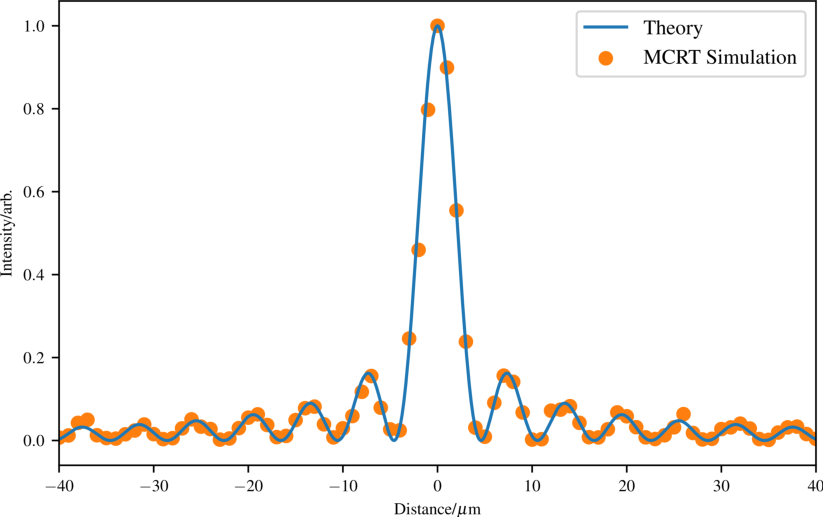
\includegraphics[width=0.65\textwidth]{compare-theory.pdf}
    \caption{Comparison of theoretical and MCRT simulation of a Bessel beams, with intensity normalised. The results from $\varphi MC$ show good agreement with the theory.}
    \label{fig:besselCompare}
\end{figure}

\begin{figure}[!htbp]
\centering
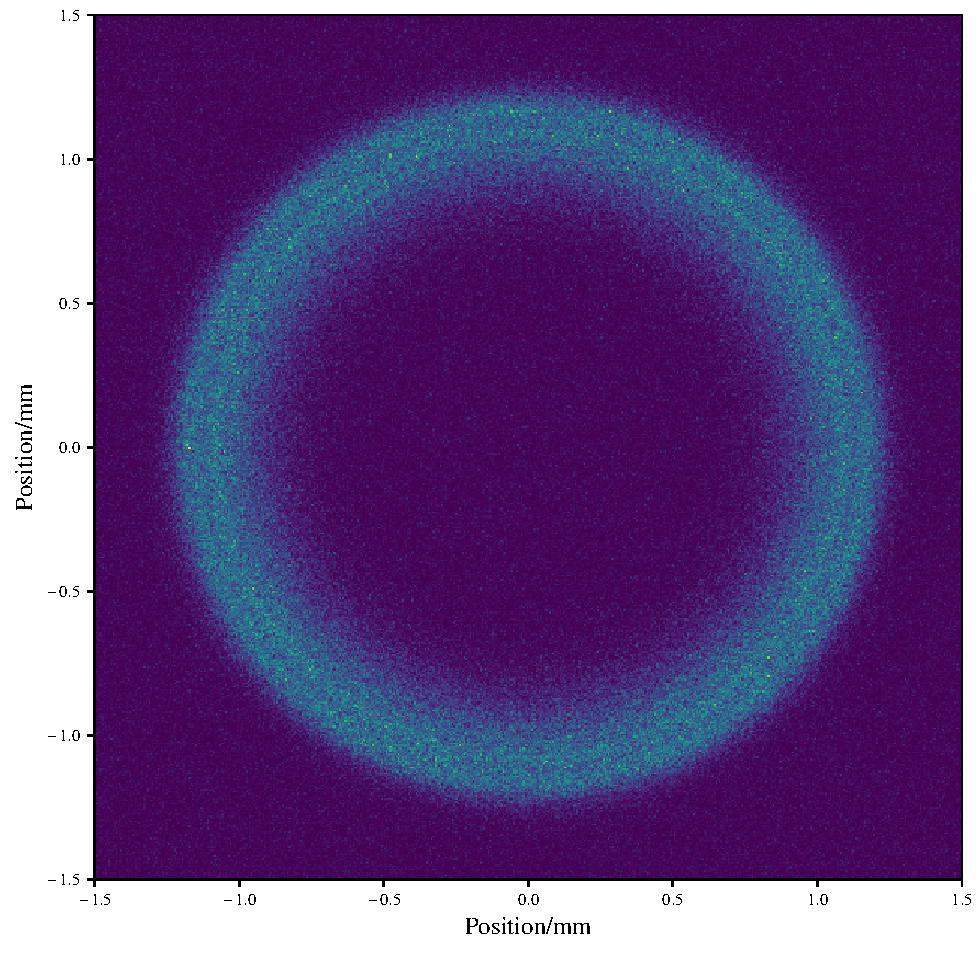
\includegraphics[width=0.5\textwidth]{farfield.pdf}
\caption{Bessel beam in the far field. Bessel beams in the far field becomes a ring beam. Image shows a slice of intensity through the medium.}
\label{fig:farfield}
\end{figure}


\subsubsection*{Comparison to experimental data}

To ensure our algorithm works in turbid media, experiments were carried out by our collaborators, S. Reidt \textit{et al.}, at the University of Dundee.
These experiments allow us to test our algorithms ability to simulate scattering of Bessel beams in turbid media.
S. Reidt \textit{et al.} carried out an experiment where a Bessel beam was propagated through a medium of varying turbidities.
A laser, wavelength $488~nm$, with a Gaussian profile is shone on an axicon lens, with angle $5^{\circ}$.
The laser beam had a $\tfrac{1}{e^2}$ diameter of $2~mm$. 


The Bessel beam was allowed to propagate through the air for $10~cm$ before entering a cuvette of side $2~mm$.
The cuvette was filled with $500~\mu L$ of water, and various volumes of a scattering agent added.
\Cref{fig:expsetup} shows the experimental set-up.
\FloatBarrier

\begin{figure}[!htbp]
\centering
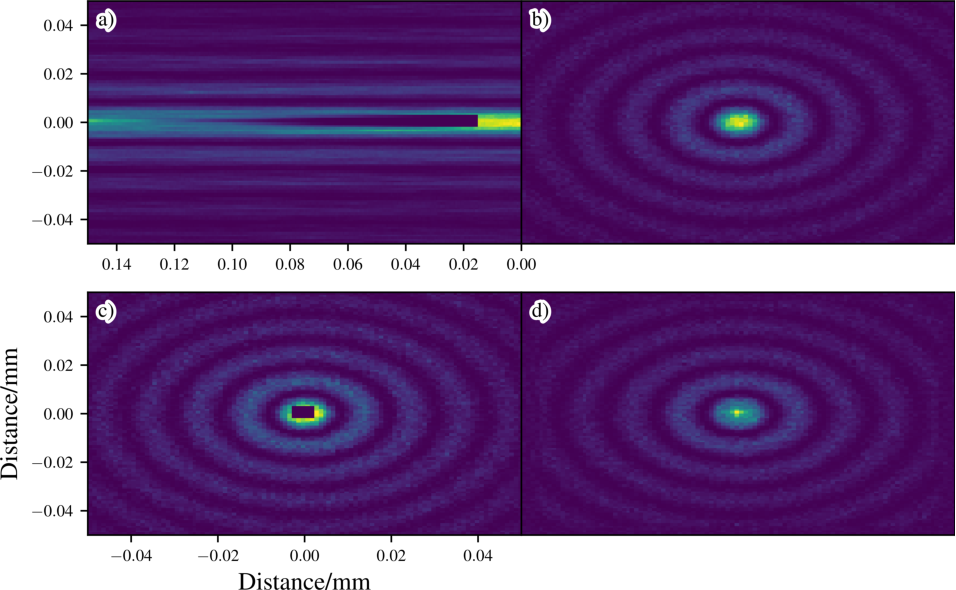
\includegraphics[width=0.75\textwidth]{selfheal.pdf}
\caption{Illustration of the Bessel beams self-healing property. Highly absorbing cube placed near the top of the medium. Figure shows that the Bessel beam forms further down the optical axis. a) shows side on view with the obstacle at $0.02~mm$, b) shows top down view at surface of the simulated b=medium before the obstacle, c) shows top down view in the middle of the obstacle, and  d) shows the top down view after the Bessel beam has ``healed''.}
\label{fig:selfheal}
\end{figure}

The scattering agent used is intralipid $20~\%$ (Sigma-Aldrich), which is diluted as shown in~\cref{tab:intra}.
~\Cref{fig:ilscatprop} shows the optical properties of Intralipid $20~\%$.
Dilutions of Intralipid are kept below 2\% scattering particle concentration, so that the scattering exhibited by the intralipid is in the independent scattering regime\footnote{The independent scattering regime is where $g$ is dependent on the size, shape and material properties of the scattering particle, and the material properties of the bulk material, but not the number of scattering particles~\cite{aernouts2013supercontinuum,mishchenko2018independent}.}.
This allows the linear scaling of the optical properties by concentrations~\cite{aernouts2013supercontinuum,vardaki2015studying,di2011effect}.
Images of the Bessel beam as it emerges from the cuvette are taken for comparison with our algorithm.


\begin{figure}[!htbp]
    \centering
    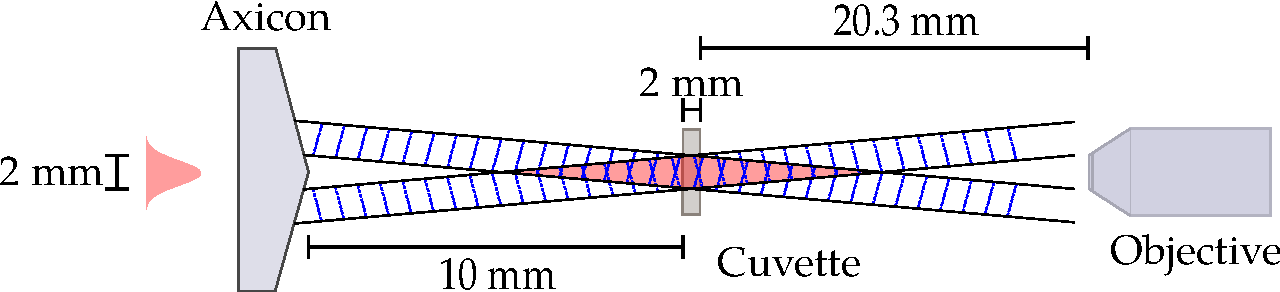
\includegraphics[width=0.8\textwidth]{bessel-exp-setup.pdf}
    \caption{Experimental set-up for propagating a Bessel beam through a cuvette filled with varying concentrations of Intralipid 20\%. Bessel beam is imaged by an $20\times$ objective lens and a Grasshopper 3 camera.}
    \label{fig:expsetup}
\end{figure}


\begin{table}[!ht]
    \begin{tabular}{cc|cc|c}
        \hline
        \multicolumn{2}{c|}{Volume/$\mu L$} & \multicolumn{2}{c|}{Intralipid concentration}                       & Optical properties              \\
        Intralipid                & $H_2O$  & Volume/\%      & Scattering particle/\%                             & Scattering coefficient/$m^{-1}$ \\ \hline
        \multicolumn{1}{c|}{0}    & 500     & \multicolumn{1}{c|}{0.00}    & 0.00                                 & 0.00                            \\
        \multicolumn{1}{c|}{2}    & 500     & \multicolumn{1}{c|}{0.39841} & 0.0908                               & 557.14                          \\
        \multicolumn{1}{c|}{4}    & 500     & \multicolumn{1}{c|}{0.79365} & 0.1816                               & 1114.28                         \\
        \multicolumn{1}{c|}{6}    & 500     & \multicolumn{1}{c|}{1.18577} & 0.2724                               & 1671.42                         \\
        \multicolumn{1}{c|}{8}    & 500     & \multicolumn{1}{c|}{1.57480} & 0.3632                               & 2228.56                         \\
        \multicolumn{1}{c|}{10}   & 500     & \multicolumn{1}{c|}{1.96078} & 0.4534                               & 2785.71                         \\
        \multicolumn{1}{c|}{12}   & 500     & \multicolumn{1}{c|}{2.34375} & 0.5448                               & 3342.84                         \\ \hline
    \end{tabular}
    \caption{Intralipid solutions used for experiment, see also~\cref{fig:ilscatprop}.}
    \label{tab:intra}
\end{table}

\begin{figure}[!htbp]
    \centering
    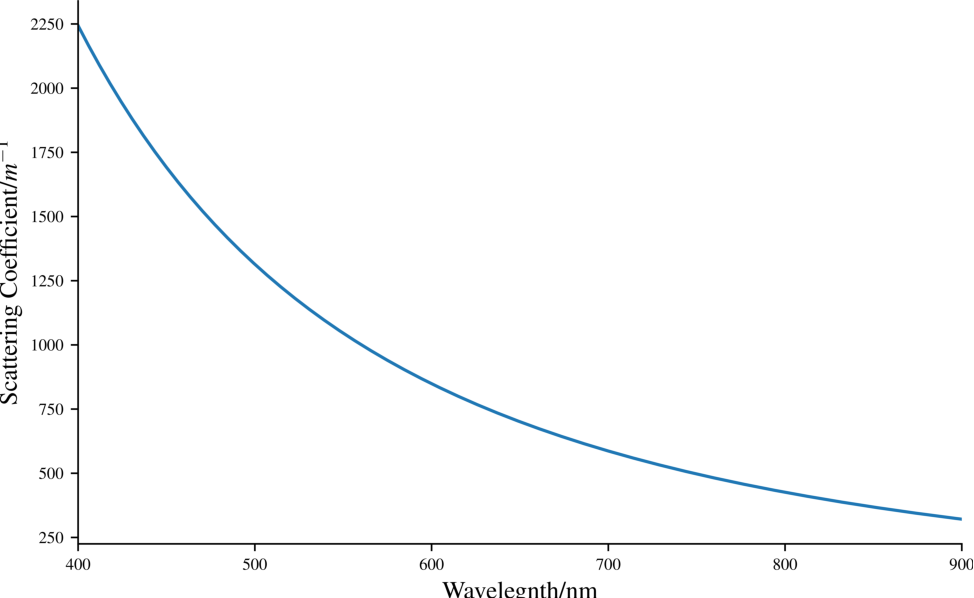
\includegraphics[width=0.5\textwidth]{scat-prop-il.pdf}
    \caption{Scattering properties of 20\% Intralipid~\cite{michels2008optical}.}
    \label{fig:ilscatprop}
    \vspace{-10pt}
\end{figure}

To model within $\varphi MC$, we simplify the experimental setup considerably.
The simulation models the propagation of photon packets through the axicon to its conical surface. 
On the conical surface the Huygens-Fresnel principle is invoked, and the packet is sampled onto the surface of the medium (cuvette).
The sampling of the photon onto the surface of the medium, speeds the algorithm up, as it does not need to simulate the photons that would ``miss'' the medium.
From there the usual~\gls*{mcrt} method propagates the packet through the medium while tracking its phase, and scattering the packet until it leaves the medium.
If the packet leaves the medium to any side other than the far side of the cuvette (e.g any side of the cuvette not facing the objective lens), then it is discarded.
If the packet leaves the medium on the objective lens facing side, then the packet is recorded by its phase onto an area element.
For each intralipid concentration $6.4\times10^{10}$ photons are run over 64 cores, taking $\sim 3$ hours for the $12\mu L$ intralipid volume.
Once all the packets have been run, the phase is converted into intensity, as in~\cref{eqn:intense}, but in 2D.

\Cref{fig:compareexpbessel,fig:compareexpbesselLine} show the results from the experiment and simulation. The simulation shows good agreement with experimental data within experimental and simulation uncertainty.

\begin{figure}[!htbp]
\centering
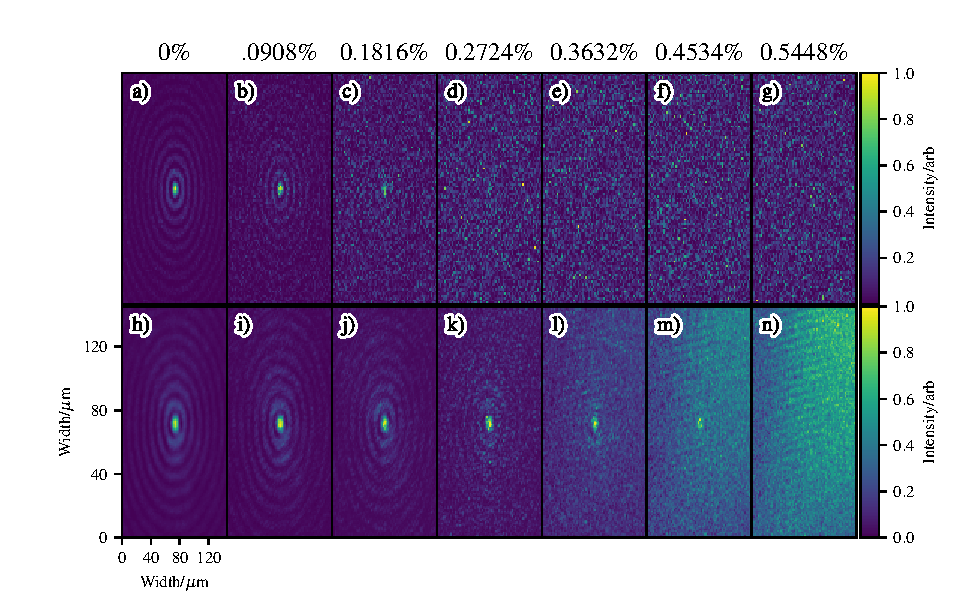
\includegraphics[width=0.95\textwidth]{compare-exp.pdf}
\caption{Comparison of experimental and simulation data for propagation of a Bessel beam produced by an axicon, through mediums of various turbidity. Images a) to g) is the data from $\varphi MC$, and h) to n) are the experimental data. Volumes along the top are the volume of Intralipid in each solution as in~\cref{tab:intra}. All images are cropped so they are the same size and normalised to the maximum value in each image.}
\label{fig:compareexpbessel}
\end{figure}

\begin{figure}[!htbp]
    \centering
    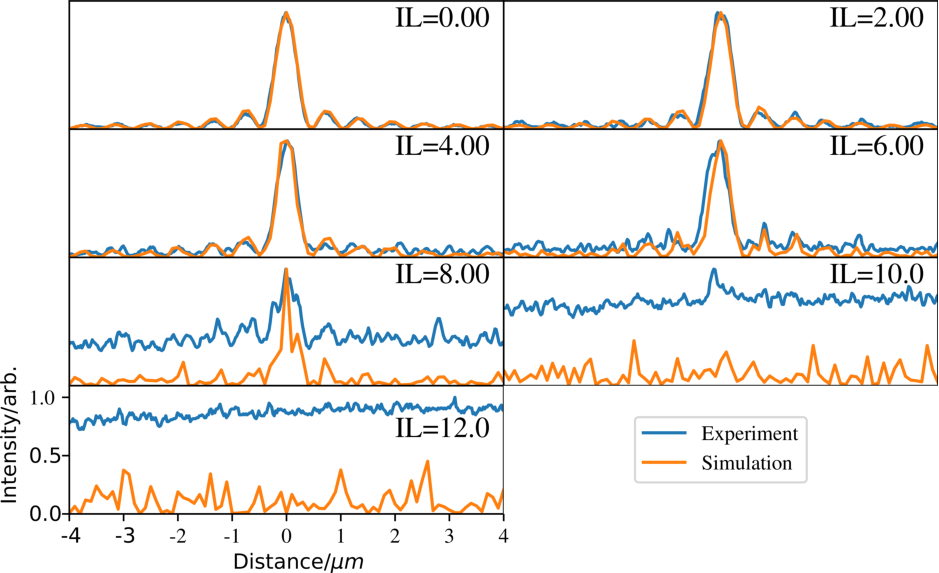
\includegraphics[width=0.75\textwidth]{Exp-sim-lineplots.pdf}
    \caption{Line graph plots of slices taken through the generated and experimental images as shown in~\cref{fig:compareexpbessel}.}
    \label{fig:compareexpbesselLine}
\end{figure}

\subsubsection*{Discussion}

As mentioned in previous sections, the power of the \gls*{mcrt} method is that we can track virtually any quantity in the simulation.
Alongside generating intensity images, we can also track the average number of scatterings per packet, a quantity that is hard to measure experimentally.
\Cref{tab:numscatt} shows the average number of scattering per packet alongside the optical depth of the medium from the source to the image plane.
The simulations show that above $\approx$ 2 scatterings of a packet the Bessel beam is ``destroyed'' and the generated image becomes washed out with noise.

\begin{table}[!ht]
    \centering
    \begin{tabular}{c|c|c}
    Volume IL/$\mu L$ & Avg \# scatterings & Optical depth \\ \hline
    2      & 0.734              & 1.114         \\
    4      & 1.225              & 2.229         \\
    6      & 1.594              & 3.342         \\
    8      & 1.899              & 4.457         \\
    10     & 2.168              & 5.571         \\
    12     & 2.417              & 6.686        
    \end{tabular}
    \caption{Average number of scattering per packet and the optical depths for different volumes of Intralipid.}
    \label{tab:numscatt}
\end{table}

Originally the medium was modelled as in the experiment, a $2~mm^3$ volume.
The image created was thus a $2001 \times 2001$ with a resolution of $1~\mu m$.
To achieve a good signal to noise ratio for this set-up $6.4\times10^{12}$ packets needed to be run, taking $\sim$ 70 hours on a computer cluster using 64 cores.
This was sufficient to get a good signal to noise ratios for all the simulations up to $6~\mu L$.
However, the number of packets needed to get a good signal to noise ratio for $8~\mu L$ and above was prohibitively computationally costly.
Therefore, the modelled medium was shrunk in the \textit{x} and \textit{y} directions giving: $0.5~mm \times 0.5~mm \times 2.0~mm$.
This allowed a smaller image (501 $\times$ 501), whilst keeping the same resolution.
Shrinking the medium also has the benefit that the photons are confined closer to the image plane, thus ensuring more photons hit the plane in comparison to the larger medium. 

Shrinking the mediums size does have some drawbacks.
First, the Bessel beams propagation depth rely on the input beams width (see~\cref{eqn:besselzmax}).
The input beams width was kept constant between the shrinking of the volumes size.
However, shrinking the mediums size in the \textit{x} and \textit{y} directions gives the same effect as using a smaller input beam.
Therefore, the \textit{x} and \textit{y} dimension were carefully chosen such that the Bessel beam would still form a Bessel beam at the image plane.
The second issue with shrinking the medium is that some packets may be lost.
This means that in the larger medium a packet may scatter toward an \textit{x} or \textit{y} medium wall and then scatter back into the centre of the medium and then is recorded.
However, this same packet in the smaller medium would be lost as the packet would exit the medium and cease to be tracked.
It is not expected that this will cause much of an issue as any scattering event already degraded the quality of the beam, as that packet is no longer coherent with the rest of the packets, thus it will not contribute positively to the Bessel beam.
To ensure this is not an issue, results from a larger medium are compared to that of the smaller medium in~\cref{fig:compareBigSmall}.
The larger and smaller medium yield the same results (within Monte Carlo noise) for Intralipid volumes less than $8~\mu L$.
At $8~\mu L$ the smaller medium has a Bessel beams central core, whilst the larger medium is noisy, and forms no Bessel beam.
This test has shown that shrinking the medium allows accurate modelling of the propagation of a Bessel beam through a turbid medium while using less computational resources.

\begin{figure}[!htbp]
    \centering
    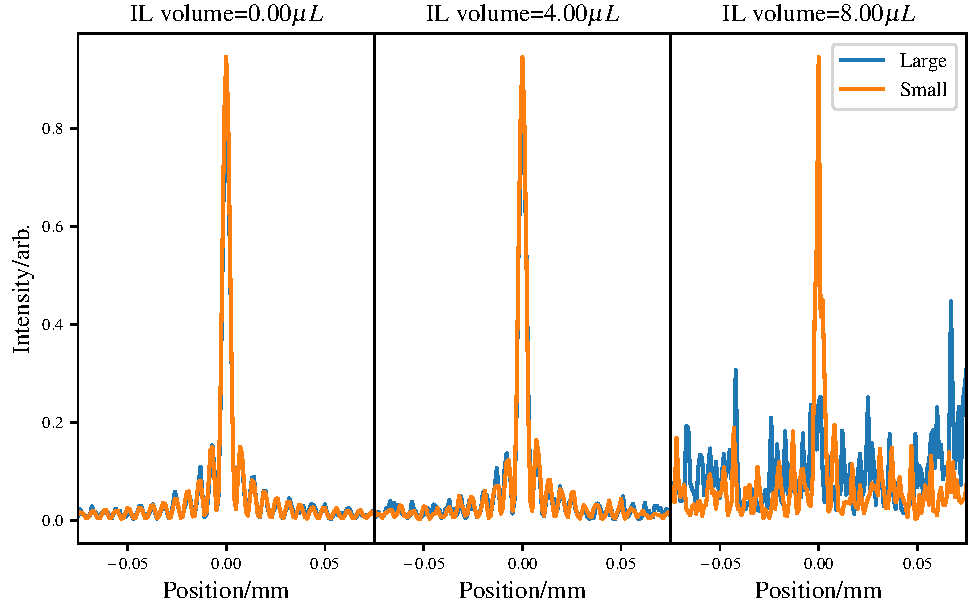
\includegraphics[width=0.7\textwidth]{compare-med-size.pdf}
    \caption{Comparison of a larger medium, $2~mm^3$ versus that of a smaller medium, $0.5~mm \times 0.5~mm \times 2.00~mm$. The figure shows that the smaller medium gives a better signal to noise ratio, whilst still accurately modelling the experiment.}
    \label{fig:compareBigSmall}
\end{figure}

\FloatBarrier

\section{Higher Order Bessel Beams}

Higher order Bessel beams (HOBBs) are Bessel beams where the electric field has an extra term of $e^{-il\varphi}$, as shown in~\cref{eqn:hobb}, and $l \neq 0$.
\Gls*{hobb} have found a use for optical trapping targets that are reflective or have a low refractive index, and optical manipulation~\cite{garces2002transfer,garces2003observation}.
Our technique outlined in the preceding sections can also be applied to arbitrary higher order Bessel beams. 

As before, the electric field of a $l^{th}$ order Bessel beam is:

\begin{equation}
E(r,\varphi,z)=E_0J_l(k_r r)e^{-i k_z z}e^{-i l \varphi}
\label{eqn:hobb}
\end{equation}

\noindent Where:

\indent $l$ is the order of the beam [-];

\indent $k_{z}^{2} + k_{r}^{2} =k^2$, where $k^2$ is the wavevector [$m^{-1}$];

\indent $r$, $\varphi$, and $z$ are the cylindrical coordinates [$m$, $rad$, $m$];

\indent and $J_l$ is the l-order Bessel function of the first kind [-].

\medskip

%properties of higher order bssel beams

%methods of generating higher orders
To generate higher order Bessel beam, a helicon is used.
A helicon (shown in~\cref{fig:helix-2}) is an axicon attached to a helix phase delay element.
The helical element imparts a helical phase delay to photon packets as they pass through the element.


The distance travelled through the helicon is shown in~\cref{eqn:helix,eqn:axicon,eqn:heightdiff}~\cite{wei2015generation}.
$h_1$ is the path length travelled by a photon through the helical element.
$h_2$ is the path through an axicon, and $\Delta h$ is the height of the helical discontinuity.

\begin{align}
h_1&=\frac{l\phi\lambda}{(n-1)2\pi} \label{eqn:helix}\\
h_2&=r\ tan(\alpha)\label{eqn:axicon}\\
h_3&=h_1+h_2 \label{eqn:helicon}\\
\Delta h &= \frac{l\lambda}{n-1}\label{eqn:heightdiff}
\end{align}

Where $\phi$ is the azimuthal angle, $r$ is the radial position, $l$ is an integer that describes the order of the Bessel beam, and $\alpha$ is the axicon angle.

The path length in the above equations can be converted into a phase delay by considering the transmission functions of the individual elements~\cite{khonina1992trochoson,kotlyar2006diffraction,topuzoski2009conversion,qiong2012generalization}:
\begin{figure}[!htbp]
    \centering
    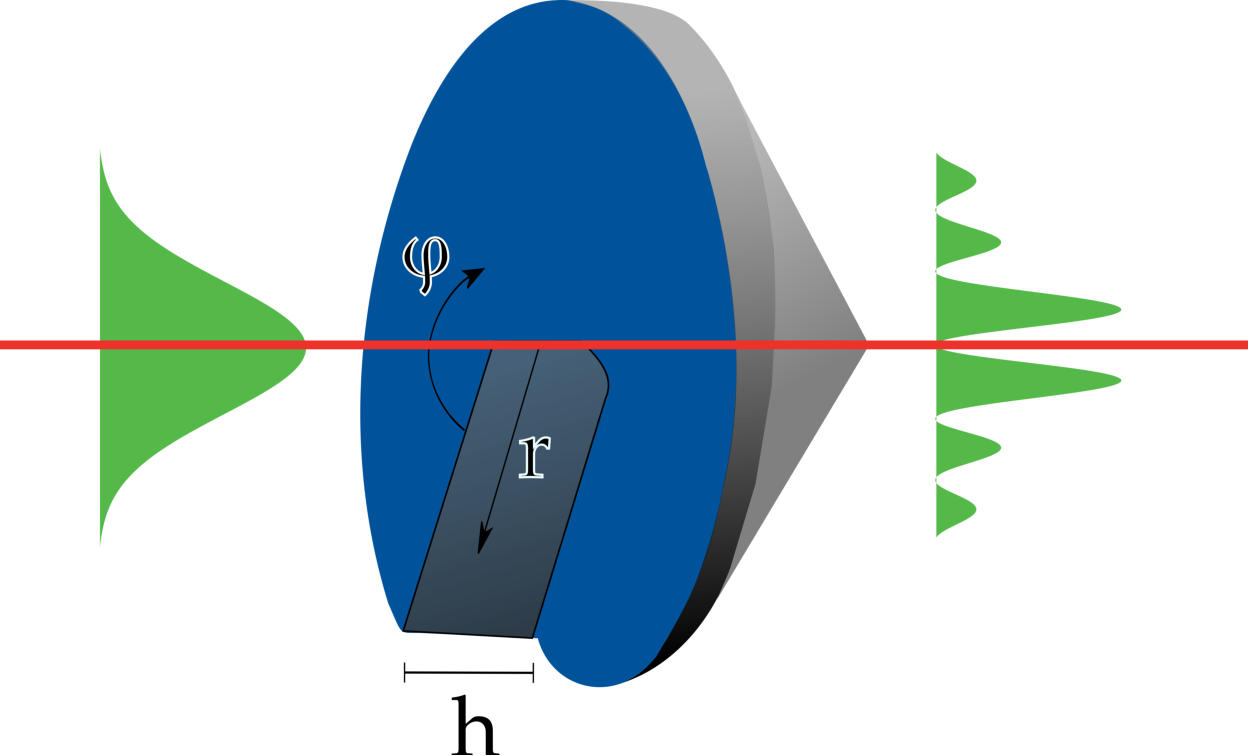
\includegraphics[width=0.4\textwidth]{helicon-2.pdf}
    \caption{Helical delay element attached to an axicon. The Axicon introduces a radial delay in addition to that of the helical element. If the input beam is a Gaussian, the output beam is a higher order Bessel beam, $l>0$.}
    \label{fig:helix-2}
    \vspace{-10pt}
\end{figure}

\begin{align}
T_1(\varphi)&=e^{-ik(n-1)h_1}=e^{-il\phi}\\
T_2(r)&=e^{-ik(n-1)h_2}=e^{-ik_rr}\\
T_3(r,\varphi)&=T_1*T_2=e^{-ik_rr-il\phi}
\end{align}

Where $T_1$ is the transmission function for the helical element, $T_2$ is the transmission function for the axicon, and $T_3$ is the total transmission function.
Using the small angle approximation  for $\beta$ and~\cref{eqn:betaangle}, and knowing $k_r=sin\left(\beta\right)$ yields the phase delay as a function of angle and radial position:

\begin{equation}
\varphi(\phi,r)=k(n-1)r\alpha+l\phi
\end{equation}

To implement a helicon in the $\varphi MC$ algorithm, a helical phase delay is added.
The additional delay is implemented by adding $l\phi$ where $0<\phi<\tfrac{2\pi}{l}$.
An actual helix element is not modelled explicitly in the code, but rather just the phase delay.
This method is similar to using a spatial light modulator in an experiment to impart a phase delay on a beam.

\Cref{fig:highordershow} shows the comparison between theoretical higher order Bessel beam and the higher order beam simulated by $\varphi MC$.

\begin{figure}[!htbp]
    \centering
    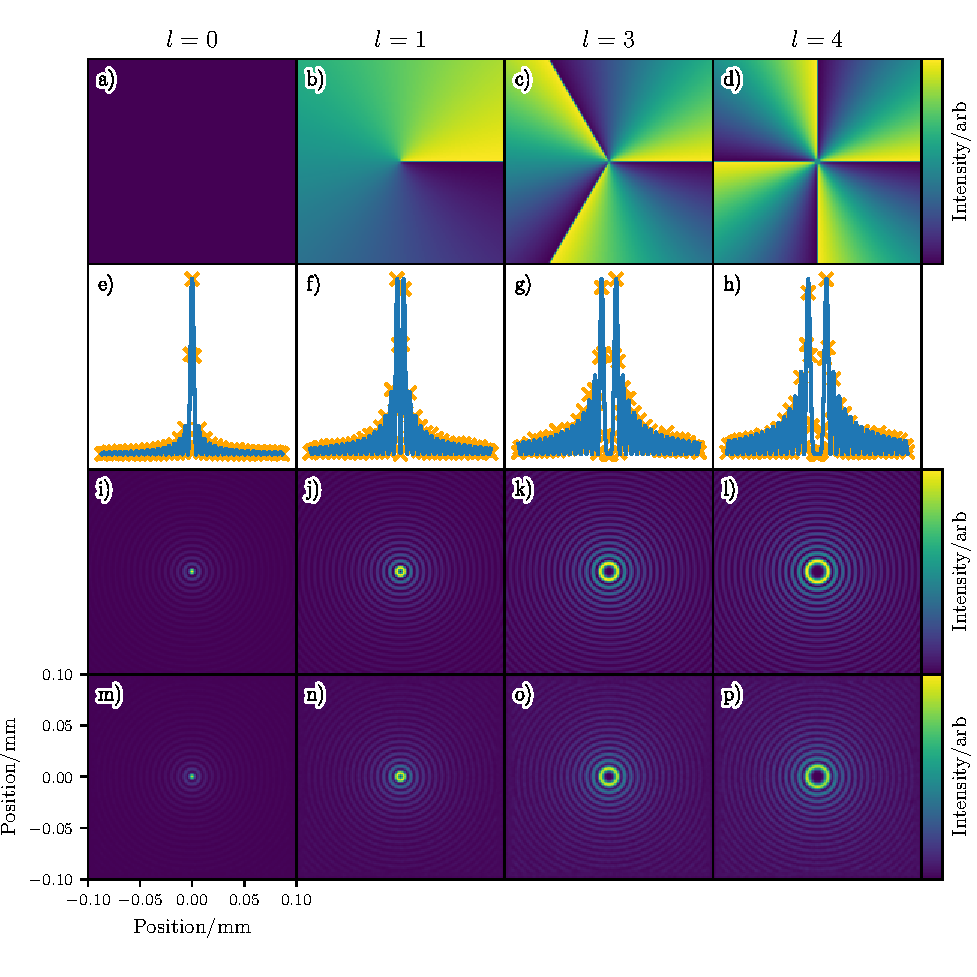
\includegraphics[width=0.85\textwidth]{higher-order-bessel.pdf}
    \caption{\Gls*{hobb}. a) to d) show the phase shift due to the helical element. e) to h) show line plots of the simulation data compared to the theory. i) to l) and m) to p) show the higher order Bessel beam images for theory and simulation data respectively.}
    \label{fig:highordershow}
\end{figure}

\FloatBarrier
\section{Comparison}
\label{sec:compBeams}
As Bessel and Gaussian beams are radically different from one another it is hard to directly compare the two beams.
Gaussian beams carry all their power in the ``central core'' of the beam, whereas in a Bessel beam, it carries the same amount of power in each ring.
Bessel beams also have a much larger depth of focus than Gaussian beams.
This section attempts to compare the two beams, to predict which beam performs better in a heavily scattering medium using $\varphi$MC\@.
Bessel beams are expected to perform better than Gaussian beams, due to their self-healing properties and non-diffractive core, this section aims to quantify how this property may or may not help penetration through a highly scattering medium. 


As mentioned, Bessel beams and Gaussian beams are not alike, so to ensure a fair comparison the Bessel beams central core width is set to that of the Gaussian beam's waist.

\begin{equation}
r_0=\frac{\kappa}{k\ sin\beta}  
\end{equation}

Where $\kappa$ is a constant that determines the metric used to measure the Bessel beam's core, and the other symbols have the same meanings as before.
For $\kappa=2.408$ the radius is measured from the maximum of the core to the first zero of the Bessel beam.
$\kappa=1.75$ measures the Bessel beam's core from the maximum to $\tfrac{1}{e^2}$ of the maximum.
For both beams central cores to be equal, the axicon used to generate the Bessel beam is adjusted.
This is achieved by calculating the ``correct'' $\alpha$ based upon the optical setup used to focus the Gaussian beam. 
Using the small angle approximation\footnote{for small $\alpha$ and $\beta$: $\beta=(n-1)\alpha$.} and $\kappa=1.75$ we can compare the Bessel beam's core radius to a Gaussian beam's waist:

\begin{align}
\frac{1.75\lambda}{2\pi sin\beta}&=\frac{2\lambda f}{\pi D} \\
\alpha &= \frac{1}{n-1}asin\left(\frac{1.75 D}{4 f}\right)
\end{align}

Where $\alpha$ is the axicon angle as before, n is the refractive index of the axicon, $D$ is the $\tfrac{1}{e^2}$ diameter of the incident Gaussian beam on the lens, and $f$ is the focal length of the lens used to focus the Gaussian beam.
Both $D$ and $f$ are properties of the optical system used to focus the Gaussian beam.
The lens used to focus the Gaussian beam is the same as used in the previous section to validate that $\varphi$MC can model a Gaussian beam, a convex-plano lens, with radius of curvature $4.6~mm$, a working distance of $8.5~mm$ and thickness of $2.2~mm$.

\medskip

The first simulation comparisons carried out between the Bessel and Gaussian beams is to use the same power to generate both beams.
The beams are then propagated through mediums of varying degrees of Intralipid solution.
Volumes of $0.0$, $26$, $52$, $78$, and $104$ $\mu L$ are used of Intralipid in 500 $\mu L$ of water.
The medium has a volume of $0.1~mm \times 0.1~mm \times 0.2~mm$, and voxel resolution of $1~\mu m$.
For both beams a wavelength of $488~nm$ and a power of $1~mW$ is used.
One hundred million packets are simulated for each simulation.
The results of this are shown in~\cref{fig:1stcomp,fig:1stcomp-1}

\begin{figure}[!htbp]
    \centering
    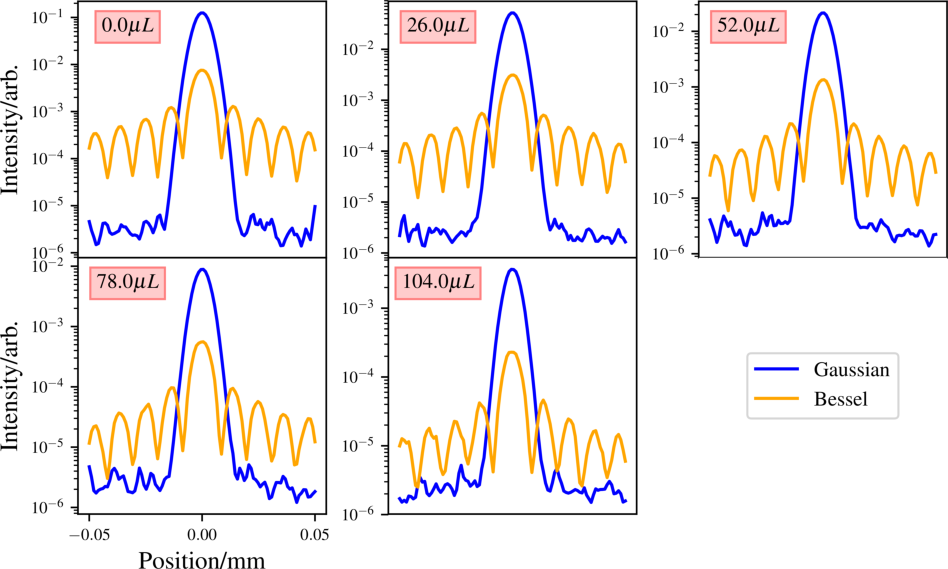
\includegraphics[width=0.75\textwidth]{Compare-BvdG-xyplane-1mW-equal-focus.pdf}
    \caption{First comparison of Bessel and Gaussian beams with equal power used to generate both beams. Plots taken at the Gaussian beams focus. The maxima at the sides of the Gaussian beam in the $0.0\mu L$ plot are due to simulation effects, mainly the small size of the medium not allowing photons from further off the optical axis to interfere destructively.}
    \label{fig:1stcomp}
\end{figure}

\begin{figure}[!htbp]
    \centering
    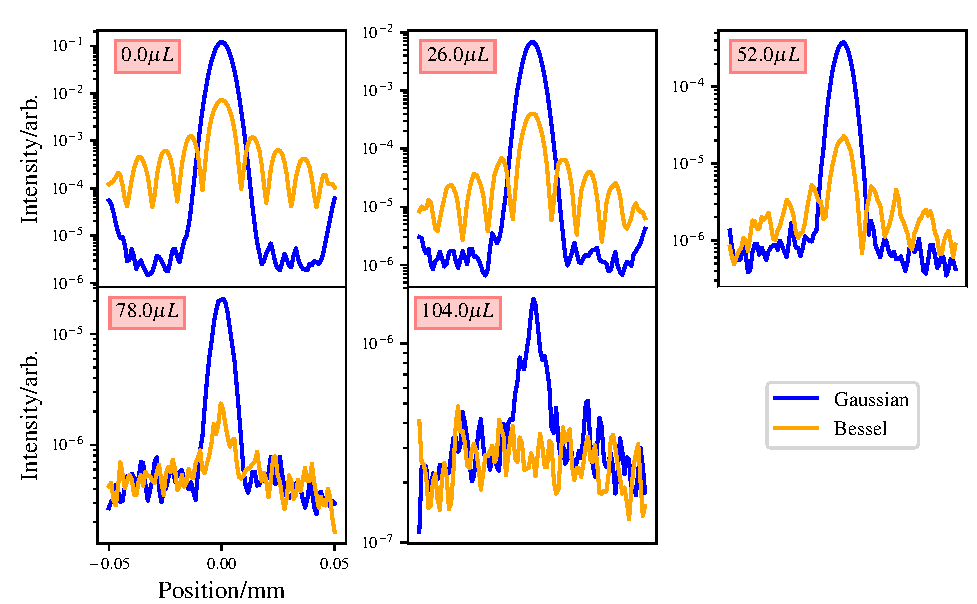
\includegraphics[width=0.75\textwidth]{Compare-BvdG-xyplane-1mW-equal-bottom.pdf}
    \caption{First comparison of Bessel and Gaussian beams, with equal power used to generate both beams. Plots taken at the bottom of the simulated medium.}
    \label{fig:1stcomp-1}
\end{figure}

The results show that for the same power, Gaussian beams propagate deeper into the medium compared to Bessel beams.
This is to be expected as in a Gaussian beam all the power is in its ``central core'', whilst the power is evenly distributed between all the Bessel beam's rings.
Therefore, for a second comparison the power given to the Bessel beam is such that the central core maximum matches that of the Gaussian beam at its focus for the case where there is no scattering.
To achieve this the Bessel beam was given $\sim 15\times$ the power given to the Gaussian beam.
The results of this comparison are illustrated in~\cref{fig:2ndcomp}.

\begin{figure}[!htbp]
    \centering
    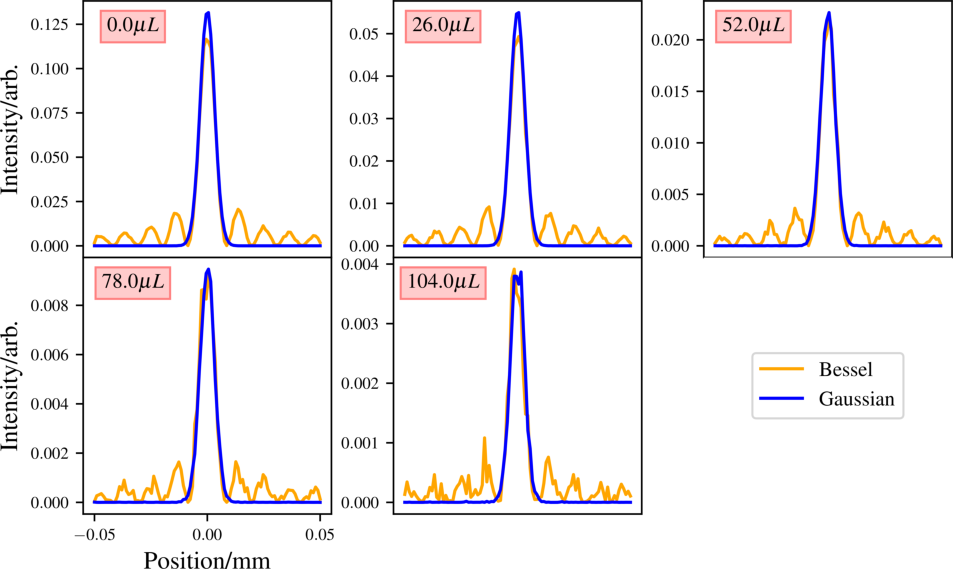
\includegraphics[width=0.75\textwidth]{Compare-BvdG-xyplane-1mW-15mW-unequal-focus.pdf}
    \caption{Second comparison of Bessel and Gaussian beams for the case where the power given to each beam, yields the same maximum at the Gaussian beams focus. These plots are taken from the Gaussian beams focus.}
    \label{fig:2ndcomp}
\end{figure}

These results show as expected that the Bessel beam now performs comparably with the Gaussian beam in lower scattering media, with a drop off in performance in the higher scattering media.

\begin{figure}[!htpb]
    \centering
    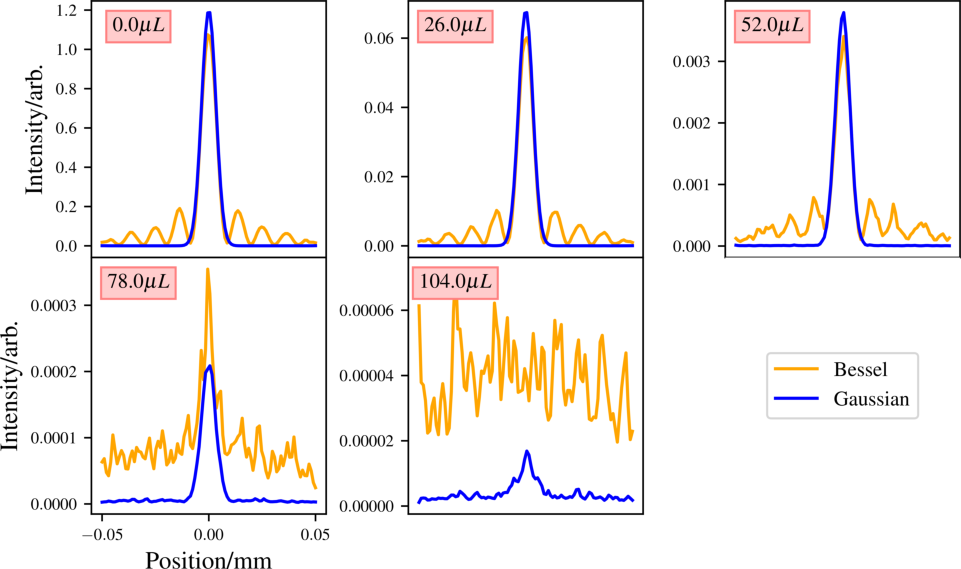
\includegraphics[width=0.75\textwidth]{Compare-BvdG-xyplane-1mW-15mW-unequal-bottom.pdf}
    \caption{Comparisons of unequal powered beams at the bottom of scattering medium.}
    \label{fig:2ncompbottom}
\end{figure}

\FloatBarrier


\subsection{Discussion}

For equal power beams in the previous section, Gaussian beams perform ``better'' in the highly scattering mediums.
Though this is expected as the power in a Bessel beam is spread evenly over its rings.
Thus, the power in the central lobe of a Bessel beam is much less than that of the Gaussian beam.

To give a slightly more fair comparison of intensity in the central lobes of the beams, the Bessel beam was given $15\times$ more power than the Gaussian beam. 
This allows a better comparison between the Gaussian beam's core and the Bessel beam's core and gives a more comparable intensity between the beam's at the location of the Gaussian beams focus.
In this case, the Bessel beam appears to perform better in a highly scattering medium, as shown in~\cref{fig:2ncompbottom}.
The Bessel beam shows comparable intensity with the Gaussian beam in the first three mediums, though the Gaussian beam out performs the Bessel beam in the higher scattering media.
It would appear that the Bessel beams self-healing property does not help a Bessel beam propagate through a highly scattering medium.
\Cref{fig:bessel-scat-explain} shows how the Bessel beam may become degraded due to scattering.
As photons propagate through the medium they interfere with one another constructively and destructively to form a Bessel beam.
However, if enough photons are scattered, then the Bessel beam becomes degraded and thus no longer is a Bessel beam, as these photons are no longer coherent with the rest of the beam, so they act as a negative factor in the beams formation.
Another reason that the ``self-healing'' property of the Bessel beam does not ``save'' the beam from scattering is that the ``self-healing'' is not self-healing.
The self-healing in reality is just photons from further off the optical axis forming the Bessel beam further down the optical axis, e.g the photons that are impeded by the blockage are stopped, but the photons that are not impeded form a Bessel beam as expected.
If you placed a blockage in front of the Bessel beam larger than the width of the input beam, then the Bessel beam would not form at all.

Bessel beams do have their positives, their self-healing property does help ``reform'' the beam past small blockages, and their depth of field is superior to an equivalent Gaussian beam, as their central core is ``non-diffractive''.


\begin{figure}[!htbp]
    \centering
    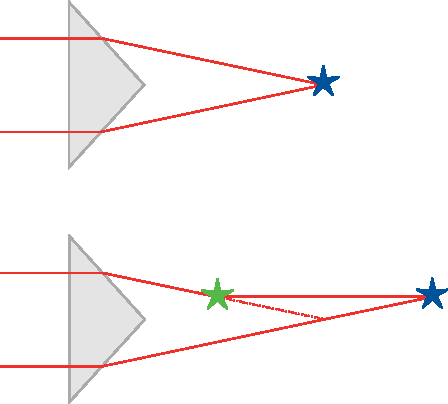
\includegraphics[width=0.5\textwidth]{bessel-scat-explain.pdf}
    \caption{Illustration of how a Bessel beam becomes degraded due to scattering. Top image shows how two photons propagate through the axicon and constructively interfere to produce a Bessel beams. Bottom image shows how scattering can affect this process.}
    \label{fig:bessel-scat-explain}
\end{figure}



\section{Conclusion}

This chapter has shown that it is possible to transform a traditional particle behaviour MCRT method into a method that allows the simulation of quasi-wave/particle behaviour of photons.
This is achieved by introducing two principles to the algorithm: the tracking of the complex phase of each packets and the Huygens-Fresnel principle.
The tracking of the complex phase of each packet allows interference of the quasi-wave/particles to be simulated.
The Huygens-Fresnel principle allows diffraction to be accurately modelled.
$\varphi MC$ has been thoroughly validated against several experiments where modelling the wave behaviour of light is vital to the experiment.
Alongside the above, presented in this chapter is the modelling of complex beam types: Gaussian and Bessel beams.
Both beam types have been validated against both theoretical and experimental results.
Finally, Gaussian beams and Bessel beams were compared with one another in a highly scattering medium, where Bessel beams appear to give better performance.
However, $\varphi$MC is not a silver bullet for modelling these complex beams in a scattering medium.
Depending on the problem at hand, the computational load can be excessive.
For example, if you want to know the intensity of the beam at all locations through a large ($> 1mm^3$) scattering medium with a complex 3D structure, then the time taken to get a good signal to noise ratio may be computationally prohibitive.
Though it is expected that in most cases the intensity is not needed at all locations in a medium, and an image is all that is needed to be calculated, then even in a complex 3D structure $\varphi$MC should perform better than the methods listed at the start of this chapter\footnote{Though to achieve better performance with the current code, adaptive mesh grids would have to be implemented.}.
Where $\varphi$MC excels is that it can accurately model scattering effects on the propagation of complex beams through scattering media.

%sources
%cizmar thesis
%born: principles of optics
%hecht: optics
%mignon
%prahl
%fresnel/fraunhoefer paper
%thorlabs
%sacsha thesis
%kishans papers
%various axicon papers
%aspheric papers
%phase screen model
%beam steering paper
%paper that hates on mcrt
%E-field mcrt